\title{Optimising HCP Sample Allocation in Pharma: Combining Nonlinear Ensemble Learning, Spatial Lags, and Integer Programming}

\begin{abstract}
Pharmaceutical companies distribute free drug samples to physicians, yet these samples frequently go to healthcare providers (HCPs) whose prescribing is unlikely to change, wasting a large share of industry-wide promotional spending. We present a framework that combines machine learning with mathematical optimisation to decide how many free samples of the anticoagulant Eliquis each HCP should receive, using historical prescribing and promotional data. We collect the prescribing behaviour of HCPs at weekly intervals; the resulting dataset comprises 2.1 years of history (109 weekly observations per HCP), totalling roughly 1.2 million provider-week records for 11,006 U.S. HCPs, together with more than 80 engineered features describing promotional activity, prescription outcomes, market share of competing and complementary therapies, patient demographics, and treatment ratios. A sparsity filter removes weak or noisy variables to improve interpretability and reduce overfitting. We then train CatBoost models, grouped into bands by prescriber value and augmented with spatial lag features that summarise how nearby providers behave, to predict the incremental gain in Total Prescriptions (TRx) and New-to-Brand prescriptions (NBRx) from additional samples; TRx measures the overall volume of prescriptions for a medication, while NBRx counts a patient's first prescription for that drug. These predictions feed a 0--1 mixed-integer programme that selects one sample quantity per HCP subject to HCP-level and territory-level pill-budget limits and operational business rules on feasibility, historical consistency, and sample availability. In a model-implied counterfactual evaluation, the spatially informed allocation increases aggregate TRx by approximately 6\%, concentrating samples on high-value providers and reducing oversupply to low-impact segments. This 6\% is a model-implied projection: realized field impact after deployment is expected to be lower, on the order of 1 to 3\%, because operational frictions, representative discretion, sample availability, and market-response uncertainty attenuate optimised recommendations. For scale, apixaban (the molecule marketed as Eliquis) accounted for roughly 19.8 million U.S. prescriptions in 2023, about 5 million per quarter \cite{ClinCalcApixaban2023}, so even single-digit efficiency gains are operationally meaningful; we report prescription-volume rather than revenue impact, as product-specific financial assumptions are outside this paper's scope. The study illustrates how spatial econometrics, machine learning, and constrained optimisation can be combined to support pharmaceutical sample-allocation planning.
\end{abstract}

\section{Introduction}\label{sec:intro}

The U.S. pharmaceutical and medical-device industry spent roughly \$30 billion on medical marketing in 2016, of which an estimated \$13--15 billion was free drug samples \cite{Schwartz2019}; this refers to industry-wide U.S. spending, not a Pfizer-specific budget. The prevailing assumption is that samples stimulate trial and loyalty, and rigorous evidence confirms they can raise new prescription starts and reshape brand choice when paired with detailing (sales representative visits to clinicians) \cite{Gonul2001,MizikJacobson2004,DonohueCevascoRosenthal2018}. Yet decades of scholarship also highlight ethical tension: grounded-theory interviews with physicians show that aggressive sampling can erode prescriber autonomy and blur professional boundaries \cite{Malik2020}, while policy debates question whether oversupply merely displaces paid prescriptions without creating genuine therapeutic value \cite{JosephMantrala2009}. These concerns motivate a shift from blanket distribution toward data-driven, patient-centric allocation.

A second motivation is economic. Even modest percentage-point gains in efficiency translate into hundreds of millions of dollars in freed-up resources \cite{Schwartz2019}. Literature reviews across nine countries consistently find that samples and face-to-face detailing dominate promotion budgets regardless of geography \cite{RajputPandey2022}, underscoring the global relevance of optimisation. Research on pandemic-era field activity further shows that pharmaceutical promotion shifted rapidly toward digital and remote channels \cite{Chiplunkar2020,KhanBasak2021}. To remain competitive, commercial teams must decide not only how many samples to drop, but where, when, and to whom: decisions that require predictive accuracy at scale.

Traditional marketing mix and nonlinear mixed-effects models impose fixed functional forms that often miss saturation points and peer spillovers \cite{MontoyaNetzerJedidi2010}. Ensemble machine learning methods such as Random Forests, LightGBM, and CatBoost can learn nonlinear saturation points and peer spillover structure with fewer a priori functional form assumptions than traditional parametric models, while retraining efficiently on large commercial data sets \cite{Chamberlain2022}. Empirical studies in healthcare confirm their superiority over classical regression for tasks ranging from rare disease targeting \cite{Cai2017} to antipsychotic prescribing prediction \cite{Antonazzoetal2022}. Nonetheless, most of the existing algorithms treat prescribers as independent units, ignoring geographic and social interdependence. A 10\% rise in a peer network's adoption rate can lift individual prescribing by 6--8\% \cite{IyengarVanDenBulteValente2011}, and clinics with high network centrality tend to prescribe fewer inappropriate medications \cite{Wangetal2023}. Spatial lag and eigenvector features reduce residual autocorrelation and cut prediction error by up to one third \cite{Liuetal2022}.

From an optimisation standpoint, free samples deliver diminishing marginal returns and sometimes negative returns at high volumes \cite{JosephMantrala2009}, while dynamic allocation policies can raise long-run profit and cut field calls by 20\% \cite{MontoyaNetzerJedidi2010}. Industry case studies echo these academic findings: IQVIA reports a 15\% reduction in oversampling after implementing breakeven analysis guided by machine learning \cite{IQVIA2025}, and an Axtria engagement found that machine learning-driven value scores re-ordered half of all targeted physicians while improving patient coverage to 95\% \cite{Awadhwal2023}. More than 70\% of life sciences firms now pilot Next Best Action engines for budget-constrained field forces \cite{MulinariOzieranski2022}.

Despite these advances, two practical gaps persist. First, most published models ignore the territorial quotas and pill-inventory caps that govern real commercial operations. Second, few studies integrate predictive modelling with a mathematically rigorous optimisation layer capable of selecting one counterfactual scenario per HCP under hard constraints. We address both gaps by leveraging 1.2 million rolling HCP--week observations for 11,006 prescribers in the eligible Pfizer call-plan universe, where each HCP--week represents a repeated weekly aggregation of prescribing and promotional activity for a given HCP across all field representatives. We construct 80+ rolling-window features and a quarterly forward indicator representing the planned sample-drop decision window used for quarterly field allocation, then train decile-banded CatBoost ensembles enriched with inverse-distance spatial lags of the optimand. Out-of-fold uplift predictions then feed a 0--1 mixed-integer programme (CBC solver with DP fallback) that enforces both HCP-level and territory-level pill bounds and operational business rules.

From a managerial standpoint, the system is intended to support quarterly sample-planning decisions about which HCPs should receive how many sample units within each territory. Recommendations are delivered at the territory level to district managers, who apportion inventory across field representatives; representatives then use those guidance values when planning office visits. Because the recommended quantities are anchored to historically observed HCP-specific ranges and territory ceilings, the outputs remain operationally defensible, easier to review, and less likely to trigger exception handling by field leadership.

Our hypothesis is straightforward: embedding spatial-peer context and hard operational constraints in a joint learning--optimisation pipeline will yield materially higher incremental TRx and NBRx than current practice using the same inventory. Future work will embed small random ``nudge'' perturbations in the final allocation plan to enable causal Difference-in-Differences estimation of real-world lift \cite{Hallettetal2024}.

In sum, this study unites ethical considerations \cite{Malik2020}, economic drivers \cite{Schwartz2019,RajputPandey2022}, predictive advances \cite{Chamberlain2022,Liuetal2022,Antonazzoetal2022}, and optimisation theory \cite{JosephMantrala2009,MontoyaNetzerJedidi2010,IQVIA2025} into a single, territory-aware framework suitable for Pfizer's North American field force, with ESG alignment defined here as reducing oversupply, preserving geographic allocation floors, and maintaining documented governance over features and allocation rules. The following sections detail our data architecture, modelling choices, optimisation formulation, and empirical results.

\section{Data}\label{sec:data}

Our modelling universe comprises about 1.2 million weekly physician--week records, giving 109 observations for each of 11,006 U.S. prescribers. All observations are merged from Pfizer's Veeva CRM call logs, IQVIA and Symphony longitudinal prescription feeds, AMA Masterfile and OneKey reference data, plus internal territory budget ledgers.

Promotional-activity predictors include lagged counts of Pfizer and BMS sample drops and channel flags indicating whether a contact occurred face-to-face or via other media. Economic theory and industry studies establish that samples and detailing raise new prescription starts but exhibit diminishing or sometimes negative marginal returns when oversupplied \cite{JosephMantrala2009,Gonul2001,DonohueCevascoRosenthal2018,MontoyaNetzerJedidi2010}.

Prescription-claims variables come from IQVIA Xponent and Symphony IDV feeds: new-to-brand and total script counts, market-basket shares for competing anticoagulants, and total-to-new-script ratios. We also derive paid-, rejected-, and reversed-claim percentages to proxy payer access, since reimbursement friction suppresses brand adoption and moderates promotional response \cite{Chiplunkar2020}. Aggregated patient demographics (age buckets and gender mix) are rolled up at the physician level; segmentation research shows that demographic mix shapes both disease prevalence and marketing elasticity \cite{Awadhwal2023}.

Geographic and peer-context features are computed as inverse-distance spatial lags of the optimand from U.S. ZIP-code centroids, following demonstrations that spatial lag and eigenvector predictors reduce model error by up to one third \cite{Liuetal2022}.

\begin{table}[ht]
  \caption{Model Feature Categories and Abstracted Variables. \textit{(Actual feature names have been anonymized for proprietary reasons.)}}
  \label{tab:variables}
  \centering
  \begin{tabular}{@{}p{0.45\linewidth} p{0.45\linewidth}@{}}
    \toprule
    \textbf{Abstract Variable Code} & \textbf{Category and Description} \\
    \midrule
    \multicolumn{2}{@{}l@{}}{\textbf{Decision Variable}} \\
    FTR\_VAR\_001 & Action variable (e.g., promotional input forecasted over 13 weeks) \\
    \midrule
    \multicolumn{2}{@{}l@{}}{\textbf{Target Optimands}} \\
    FTR\_VAR\_002 & Target outcome variable A (e.g., predicted behavior over 13 weeks) \\
    FTR\_VAR\_003 & Target outcome variable B (alternative target of interest) \\
    \midrule
    \multicolumn{2}{@{}l@{}}{\textbf{Historical Inputs}} \\
    FTR\_VAR\_004 to FTR\_VAR\_007 & Historical activity counts (past 9--52 weeks) \\
    \midrule
    \multicolumn{2}{@{}l@{}}{\textbf{Channel Flags \& Visit Types}} \\
    FTR\_VAR\_008 to FTR\_VAR\_020 & Face-to-face and remote channel indicators by segment \\
    \midrule
    \multicolumn{2}{@{}l@{}}{\textbf{Provider Attributes}} \\
    FTR\_VAR\_021 to FTR\_VAR\_023 & Experience, specialty type, high-engagement flags \\
    \midrule
    \multicolumn{2}{@{}l@{}}{\textbf{Claims Quality Metrics}} \\
    FTR\_VAR\_024 to FTR\_VAR\_025 & Percent of paid and rejected claims \\
    \midrule
    \multicolumn{2}{@{}l@{}}{\textbf{Market Share Indicators}} \\
    FTR\_VAR\_026 to FTR\_VAR\_029 & Competing or complementary brand volumes \\
    \midrule
    \multicolumn{2}{@{}l@{}}{\textbf{Patient Demographics}} \\
    FTR\_VAR\_030 to FTR\_VAR\_037 & Age bands and gender mix by condition \\
    \midrule
    \multicolumn{2}{@{}l@{}}{\textbf{Treatment Ratios}} \\
    FTR\_VAR\_038 to FTR\_VAR\_040 & Treatment-to-diagnosis and response ratios \\
    \midrule
    \multicolumn{2}{@{}l@{}}{\textbf{Exclusion Flags}} \\
    FTR\_VAR\_041 to FTR\_VAR\_043 & Specialty exclusion, global exclusion, override flags \\
    \bottomrule
  \end{tabular}
\end{table}

\section{Methods}\label{sec:methods}

Figure~\ref{fig:pipeline_schematic} summarises the end-to-end pipeline from rolling-window panel construction through banded response estimation, constrained optimisation, top-off, and final field-pack generation.

\begin{figure}[ht]
  \centering
  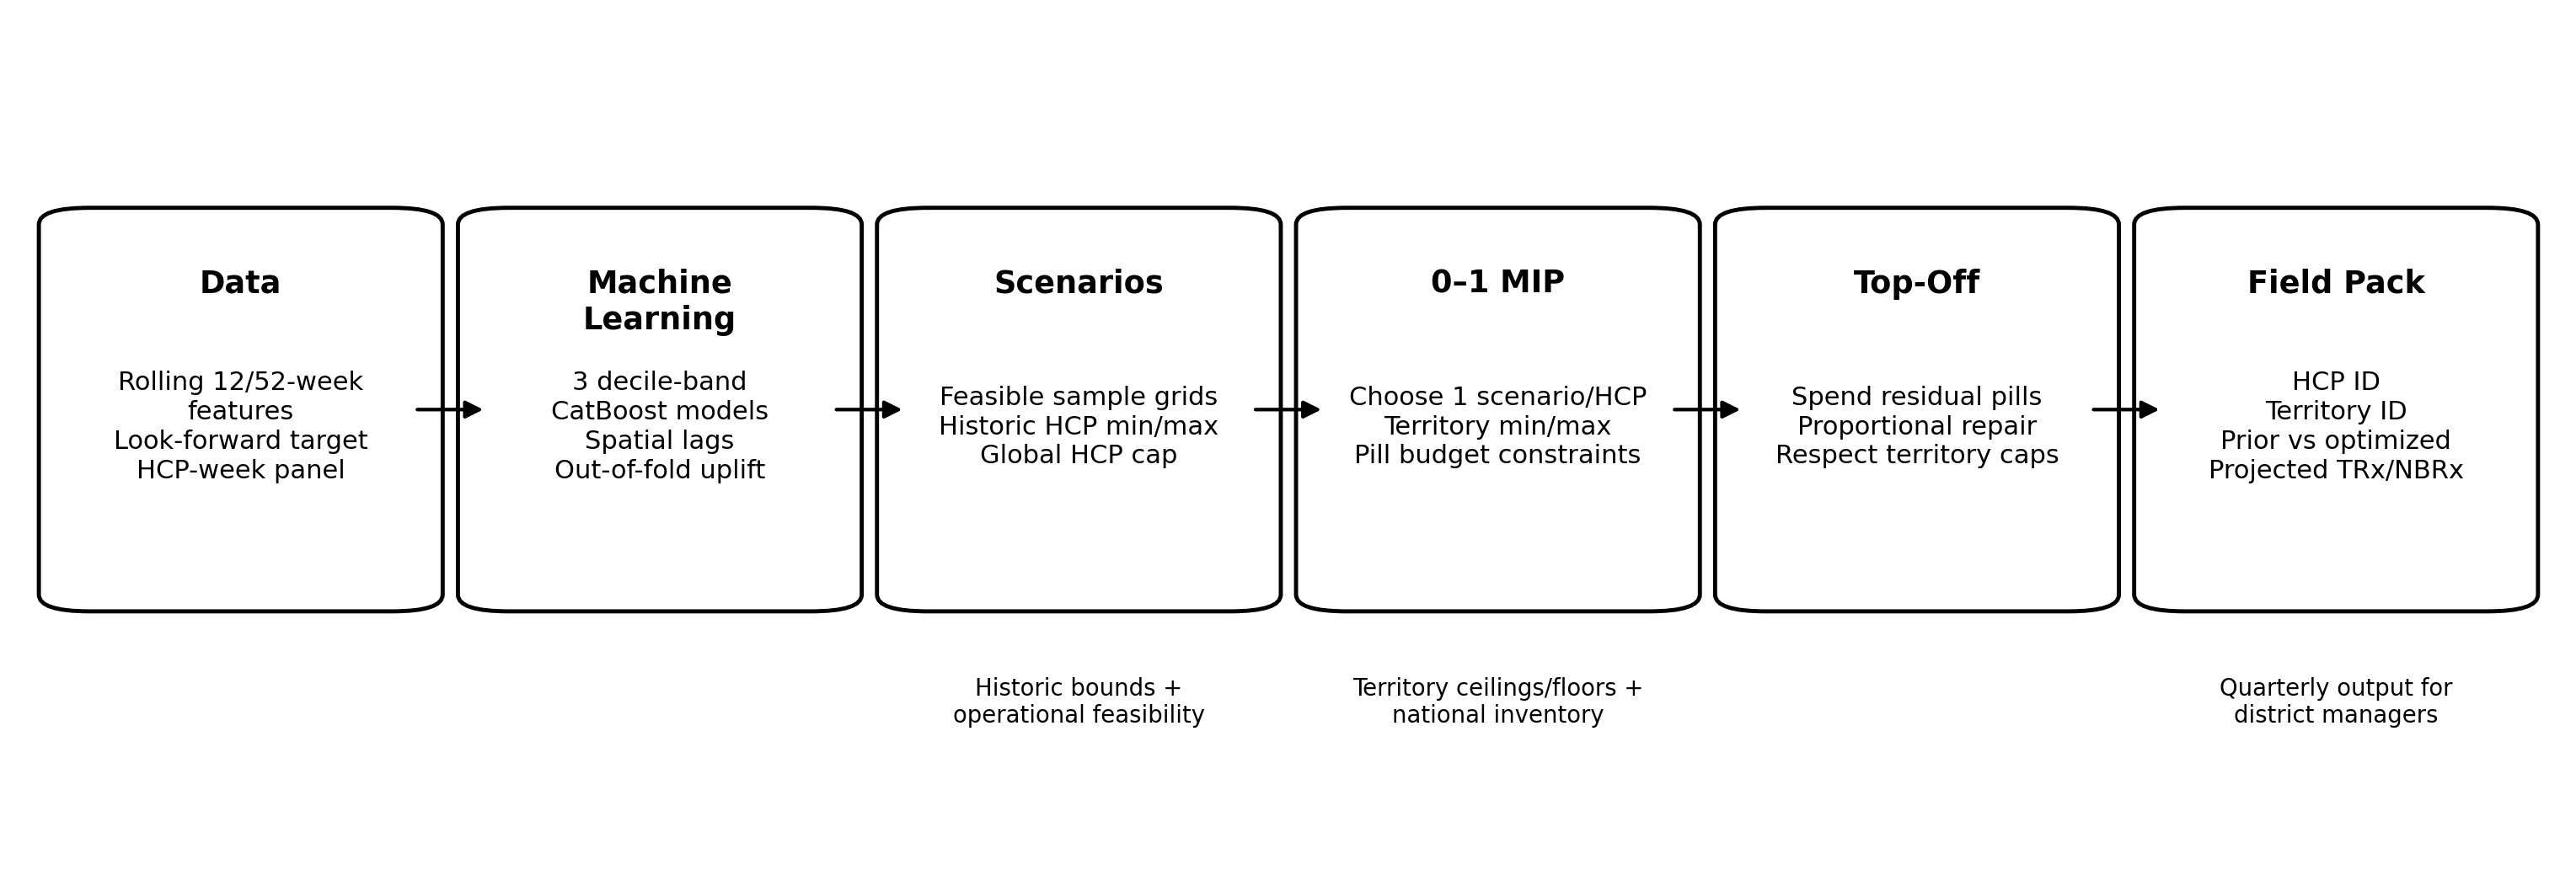
\includegraphics[width=\linewidth]{figures/figure_pipeline_schematic.png}
  \caption{Pipeline schematic for the proposed framework. Data engineering constructs rolling-window HCP-level predictors and look-forward outcomes; machine learning models estimate band-specific response surfaces; scenario generation creates feasible HCP-level sample choices subject to historical and operational bounds; the mixed-integer program selects one scenario per HCP under HCP-level and territory-level constraints; a top-off heuristic spends residual inventory; and the final field pack reports HCP ID, territory ID, prior allocation, optimized allocation, and projected response.}
  \label{fig:pipeline_schematic}
\end{figure}

\subsection{Training Data Preparation}

We extract the raw observational panels for each HCP from Pfizer's North American commercial data environment and perform upstream filtering, joins, and aggregation before modeling. The resulting analysis tables are then transferred into Python for feature engineering and estimation \cite{RahmanMueller2021,Chamberlain2022}.

Two binary indicators, \texttt{IS\_TRX\_ZERO} and \texttt{IS\_SAMPLES\_ZERO}, are created in-database. For every healthcare provider \(i\) observed over \(T_i\) weeks we compute
\begin{equation}\label{eq:sparsity}
\bar r_i
= \frac{1}{3T_i}
  \sum_{t=1}^{T_i}\Bigl[
    \mathrm{IS\_TRX\_ZERO}_{it}
    + \mathrm{IS\_SAMPLES\_ZERO}_{it}
    + \mathbf{1}\{\text{both}=1\}
  \Bigr],
\end{equation}
and retain only those panels whose average sparsity \(\bar r_i\) does not exceed \(r^* = 0.30\). Panels shorter than the minimum length \(T_{\min}=100\) are dropped, and no more than \(R_{\max}=1.2\) million unique provider-week records are processed in a single run. Randomised batching (500 IDs per chunk) prevents memory spikes while the global row limit guarantees that downstream feature engineering remains in-core.

\begin{figure}[ht]
  \centering
  
\includegraphics[width=0.8\linewidth]{figures/figure1.png}
  \caption{Sparsity of optimand and decision-variable data.}
  \label{fig:sparsity_combined}
\end{figure}

Ratio \(a\), the share of sample-drop records equal to zero, and ratio \(b\), the share of TRx records equal to zero, gauge each provider's inactivity in drops or prescriptions, while ratio \(c\), the joint zero-rate, identifies the sparsest panels. During sampling we drop any HCP whose ratio \(c\) exceeds \(r^*\), and we stratify/batch providers by the distributions of ratios \(a\) and \(b\) so the training set spans from highly active to moderately sparse panels (Figs.~\ref{fig:sparsity_decision} and \ref{fig:optimand_sparsity}).

\begin{figure}[ht]
  \centering
  
\includegraphics[width=0.65\linewidth]{figures/figure2.png}
  \caption{Decision-variable sparsity.}
  \label{fig:sparsity_decision}
\end{figure}

\begin{figure}[ht]
  \centering
  \begin{subfigure}[b]{0.48\textwidth}
    
\includegraphics[width=\linewidth]{figures/figure3a.png}
    \caption{TRx sparsity.}
    \label{fig:optimand_sparsity_trx}
  \end{subfigure}
  \begin{subfigure}[b]{0.48\textwidth}
    
\includegraphics[width=\linewidth]{figures/figure3b.png}
    \caption{NBRx sparsity.}
    \label{fig:optimand_sparsity_nbrx}
  \end{subfigure}
  \caption{Optimand variable sparsity (TRx and NBRx).}
  \label{fig:optimand_sparsity}
\end{figure}

\subsection{Response Transformation}

The response variable \texttt{growth\_score} exhibits extreme right-tail skewness. A log-plus-one transform,
\[
  y^{\log} = \log(1 + y),
\]
normalises the distribution and stabilises variance. Because the transform re-centres the target, no additional standardisation is applied. CatBoost fits and predicts on the log scale; values are exponentiated only for final business reporting, satisfying the recommendation for heavy-tailed targets in applied statistics \cite{OsborneWatkins2019}.

\begin{figure}[ht]
  \centering
  \begin{subfigure}[b]{0.48\textwidth}
    
\includegraphics[width=\linewidth]{figures/figure4a.png}
    \caption{TRx distribution.}
    \label{fig:optimand_dist_trx}
  \end{subfigure}
  \begin{subfigure}[b]{0.48\textwidth}
    
\includegraphics[width=\linewidth]{figures/figure4b.png}
    \caption{NBRx distribution.}
    \label{fig:optimand_dist_nbrx}
  \end{subfigure}
  \caption{Optimand variable distributions (TRx and NBRx) before log-plus-one transform.}
  \label{fig:optimand_distribution}
\end{figure}

\subsection{Panel Construction, Feature Engineering, \& Spatial Equity}

Feature engineering proceeds in three passes:
\begin{enumerate}
  \item Convert component counts \(x_{ijk}\) to shares
    \[
      \mathrm{perc}_{ijk}
        = \frac{x_{ijk}}{\sum_{j=1}^K x_{ij}}
    \]
  \item Expand categorical descriptors with \texttt{OneHotEncoder(drop="first")}, and \(z\)-score continuous covariates via \texttt{StandardScaler}, both fitted on training folds only \cite{Pedregosa2011}.
  \item Add spatial context by computing inverse-distance spatial lags of the optimand for every timestamp. These spatial weights approximate a composite of inter-HCP referral topology and physical distance, capturing spillovers from nearby and clinically connected peers while reducing residual autocorrelation \cite{Liuetal2022}; see Figure~\ref{fig:spatial_topology}. Because the allocation problem is inherently spatially referenced, these same features also permit map-based review of recommendations at the territory level during field-planning discussions. In line with our governance posture, feature inclusion is further constrained by sparsity filtering, predictive relevance, and documented review so that only variables with demonstrable signal and a clear business justification are retained.
\end{enumerate}

\subsection{Spatial Geometry \& Lagging}\label{sec:spatial}

We integrate territory call-list data by issuing a lightweight Snowflake SQL session that runs a multi-CTE query to filter on reference dates, deduplicate HCP rows, and compute per-territory quarterly and annual call totals, percentages, and pill quotas. The resulting table, containing \texttt{PFZ\_CUST\_ID}, \texttt{TERR\_CD}, \texttt{GEOGRAPHY}, \texttt{TERR\_OD}, \texttt{PRCT\_OD}, \texttt{TERR\_MAX}, and \texttt{TERR\_MIN}, is merged into our cleaned panel on \texttt{PFZ\_CUST\_ID}, and any missing territory codes are logged and removed. We then enrich this merged panel with dissolved territory geometries and attach standardized GEOGRAPHY names and polygon shapes to each HCP row. Finally, inverse-distance spatial lags of the optimand are computed at each timestamp by taking the dot product \( W_t y_t \), where \( W_t \) denotes the spatial weights matrix and \( y_t \) the panel of optimand values. This transforms geographic context into continuous predictors that mitigate residual autocorrelation and enhance model performance \cite{DellaVignaGentzkow2019}.

Hence, to model spatial spillover effects, we introduce a lagged version of the optimand, computed weekly for each provider:
\[
  y^{(\mathrm{spatial\;lag})}_{it}
    \;=\;
    \sum_{j \in \mathcal{N}(i)} w_{ij}\,y_{jt},
  \quad
  \sum_{j} w_{ij} = 1,
\]
where \(\mathcal{N}(i)\) is the set of spatial neighbors of provider \(i\) and \(w_{ij}\) are the row-standardised inverse-distance weights, normalized to sum to one. This lag term captures externalities in treatment behavior: providers in adjacent regions may respond similarly to market dynamics, competitive pressure, or institutional norms. Including the lagged optimand improves generalisation by accounting for spatial autocorrelation, a known confounder in healthcare outcomes research \cite{Wangetal2023}. The resulting predictor sharpens model accuracy and aligns with econometric best practices for spatially referenced data, while also enabling GIS-based review of territory-level recommendation clusters during operational planning.

\begin{figure}[ht]
  \centering
  
\includegraphics[width=0.8\linewidth]{figures/figure5.png}
  \caption{Distribution of lagged optimand.}
  \label{fig:lagged_optimand}
\end{figure}

\subsection{Spatial Autocorrelation Analysis}

Each provider is linked to a geographic unit, typically a sales territory, by joining their \texttt{PFZ\_CUST\_ID} to the Territory Call List (TCL), a canonical mapping produced by the field planning team. We then overlay this mapping with a precomputed spatial weights matrix, based on geospatial contiguity or centroid distance, to calculate spatial lags of the optimand for each week. These lagged values represent the average behavior of geographically proximate peers and are included as continuous predictors in the final model.

Spatial lags are motivated by empirical evidence in regional science and marketing analytics showing that nearby agents often respond similarly to interventions or market forces. In our use case, healthcare providers in adjacent territories may be influenced by shared sales representatives, institutional affiliations, or regional policy shifts. Including the lagged optimand thus allows the model to adjust for correlated behavior and unobserved spatial shocks, reducing residual autocorrelation and improving predictive accuracy.

Table~\ref{tab:spatial_nbrx} presents the results of Moran's I and Getis-Ord G* statistics for the NBRx optimand and the Pfizer sample-drop forecast. Table~\ref{tab:spatial_trx} does the same for the TRx optimand.

\begin{table}[ht]
  \centering
  \caption{Spatial Autocorrelation for NBRx Variables}
  \label{tab:spatial_nbrx}
  \small
  \begin{tabular}{@{}lrrrrrrrrrr@{}}
    \toprule
    \textbf{Variable} & \textbf{Moran's I} & $E[I]$ & $Z$ & $p$ & \textbf{Reject?} & $G_{\mathrm{obs}}$ & $E[G]$ & $Z$ & $p$ & \textbf{Reject?} \\
    \midrule
    \texttt{FTR\_SAMPLE\_DROPPED\_PFIZER\_FW\_1\_13W} mean
      & $-0.01885$ & $-0.00219$ & $-0.7685$ & $0.4422$ & No
      & $0.01751$ & $0.01751$ & $0.0219$ & $0.9825$ & No \\
    \texttt{TGT\_NBRX\_ELIQUIS\_ALL\_COUNT\_FW\_1\_13W} mean
      & $-0.04979$ & $-0.00219$ & $-2.1948$ & $0.0282$ & Yes
      & $0.01739$ & $0.01751$ & $-1.2279$ & $0.2195$ & No \\
    \bottomrule
  \end{tabular}
\end{table}

\begin{table}[ht]
  \centering
  \caption{Spatial Autocorrelation for TRx Variables}
  \label{tab:spatial_trx}
  \small
  \begin{tabular}{@{}lrrrrrrrrrr@{}}
    \toprule
    \textbf{Variable} & \textbf{Moran's I} & $E[I]$ & $Z$ & $p$ & \textbf{Reject?} & $G_{\mathrm{obs}}$ & $E[G]$ & $Z$ & $p$ & \textbf{Reject?} \\
    \midrule
    \texttt{FTR\_SAMPLE\_DROPPED\_PFIZER\_FW\_1\_13W} mean
      & $-0.02984$ & $-0.00218$ & $-1.2769$ & $0.2016$ & No
      & $0.01721$ & $0.01747$ & $-1.8178$ & $0.0691$ & No \\
    \texttt{TGT\_TRX\_ELIQUIS\_ALL\_COUNT\_FW\_1\_13W} mean
      & $0.01634$ & $-0.00218$ & $0.8553$ & $0.3924$ & No
      & $0.01757$ & $0.01747$ & $0.8159$ & $0.4146$ & No \\
    \bottomrule
  \end{tabular}
\end{table}

For NBRx, the Moran's I statistic for the target variable is significant (\(p=0.028\)), suggesting weak but statistically relevant spatial autocorrelation and justifying the inclusion of spatial lags in predictive modeling. By contrast, the TRx optimand did not exhibit significant spatial autocorrelation (\(p=0.39\)), indicating a more diffuse or independent pattern. Neither case showed significant Getis-Ord G* clustering for the sample-drop variable, implying no current geographic bias in sampling.

\begin{figure}[ht]
  \centering
  
\includegraphics[width=0.65\linewidth]{figures/figure6.png}
  \caption{Decision-variable choropleth.}
  \label{fig:decision_choropleth}
\end{figure}

\begin{figure}[ht]
  \centering
  \begin{subfigure}[b]{0.48\textwidth}
    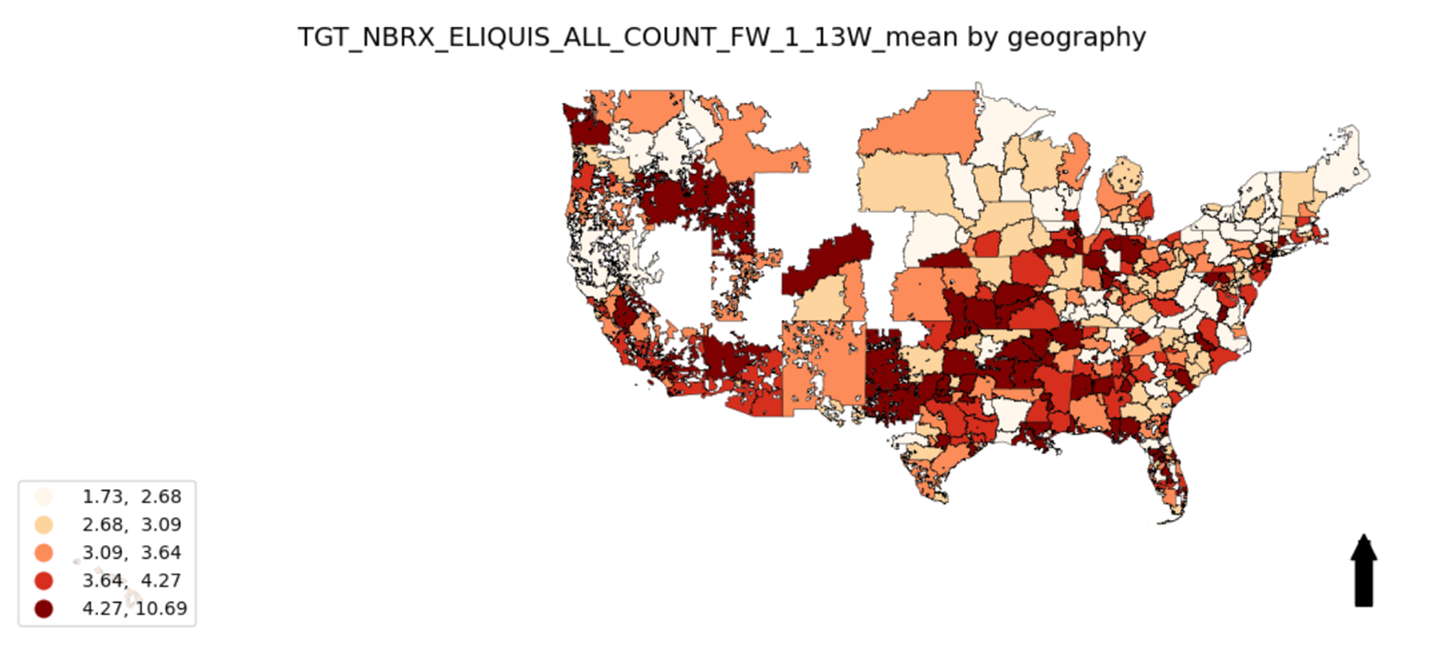
\includegraphics[width=\linewidth]{figures/figure7a.png}
    \caption{TRx choropleth.}
    \label{fig:optimand_choropleth_trx}
  \end{subfigure}
  \begin{subfigure}[b]{0.48\textwidth}
    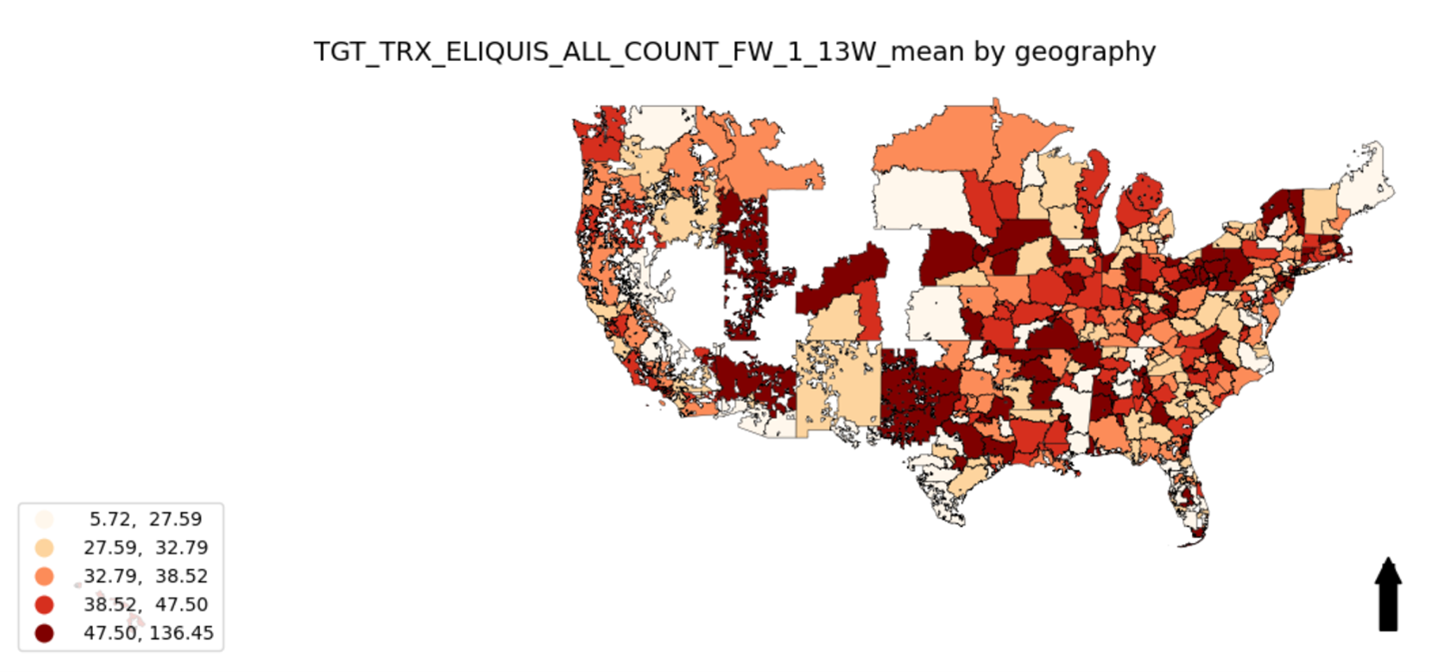
\includegraphics[width=\linewidth]{figures/figure7b.png}
    \caption{NBRx choropleth.}
    \label{fig:optimand_choropleth_nbrx}
  \end{subfigure}
  \caption{Optimand variable choropleths for NBRx (left) and TRx (right).}
  \label{fig:optimand_choropleth}
\end{figure}

\subsection{Territorial Constraints}\label{sec:territorial}

To enforce business constraints tied to field execution, we incorporate territorial ceilings and floors derived from Pfizer's Smart Targeting system. These upstream optimisations generate territory-level optimal detailing counts that guide how pill budgets are to be distributed across geographies. By aggregating observed call volumes and aligning them to these optimal detailing benchmarks, we derive the constraints \(U_t\) and \(L_t\), representing the maximum and minimum sample allocations for territory \(t\), respectively. The ceilings are computed as
\[
  U_t = p_t\,P_{\mathrm{adj}},
\]
where \(p_t\) is the proportion of national detailing activity accounted for by territory \(t\). The territory-level minimum \(L_t\) (called \texttt{TERR\_MIN} in the SQL) is set conservatively to
\[
  L_t = \max\{1,\;\lvert\mathcal H_t\rvert\},
\]
where \(\mathcal H_t\) denotes the set of distinct HCPs assigned to territory \(t\), and the constant 1 enforces a hard floor of one sample-drop unit in any territory, even those with only one HCP.

The variance of Smart Targeting's optimal detailing recommendations is empirically observed to lie within a 1 to 3\% band (a property of the upstream benchmark, unrelated to the projected uplift reported later). This tight variance range acts as a de facto regularisation mechanism, constraining the optimisation's feasible region and ensuring that pill allocations remain congruent with the original intent of Smart Targeting. The effect is to preserve geographic equity while still allowing for localised optimisation, and to guarantee that no territory's sample drop count diverges materially from historically validated expectations \cite{Awadhwal2023}.

These form the territorial constraints for our mixed-integer programme that will be formalized in a later section:

\paragraph{Territory constraints}
\[
  L_t \;\le\; \sum_{h\in\mathcal H_t} s_h \;\le\; U_t,
  \quad\forall\,t\in\mathcal T.
\]

\paragraph{Global budget (static)}
\[
  \sum_{h} s_h \;\le\; P_{\mathrm{adj}}.
\]

\paragraph{Per-HCP bounds}
\[
  0 \;\le\; s_h \;\le\; S_{\max},
  \quad\forall\,h.
\]

Two disjoint HCP subsets never enter the optimiser:
\begin{enumerate}
  \item \emph{Unaligned} HCPs lacking a valid territory ID or geography. Let \(n_{\mathrm{unaligned}}\) denote their count.
  \item \emph{Aligned but unmatched} HCPs present in the TCL yet absent from the scenario panel; call this \(n_{\mathrm{unmatched}}\).
\end{enumerate}

With \(m\) pills per HCP we deduct
\[
  P_{\mathrm{exc}}
    = (n_{\mathrm{unaligned}} + n_{\mathrm{unmatched}})\,m,
  \quad
  P_{\mathrm{adj}}
    = P_{\mathrm{tot}} - P_{\mathrm{exc}}.
\]
The pill-budget adjustment routine below (\texttt{compute\_adjusted\_pills} in code) guarantees no double-deduction.

\paragraph{Territory Unaligned and Aligned Unison: Pill-Budget Adjustment.}
\begin{enumerate}
  \item Pull full TCL with \texttt{PFZ\_CUST\_ID}, \texttt{TERR\_CD}, \texttt{GEOGRAPHY}.
  \item Count unaligned rows (nulls or literal ``NaN'').
  \item If a scenario panel is supplied, count aligned IDs missing therein.
  \item Return \((P_{\mathrm{exc}},P_{\mathrm{adj}})\).
\end{enumerate}

\section{Algorithm Overview and Development}

\subsection{Growth Model Ensemble}

Model development begins once the cleaned, spatially enriched panel has been split into mutually exclusive training and test folds with a group-aware shuffle that prevents the same prescriber from leaking across folds. All continuous covariates are \emph{z}-scored on the training fold only, while categorical descriptors are expanded with a one-of-\(K\!-\!1\) design matrix.

\paragraph{Notation.}
Let \(\mathbf X_b\in\mathbb R^{n_b\times p}\) denote the design matrix for band \(b\) with \(p\approx600\) one-hot-expanded features, and let \(y_{it}\) be the log-plus-one target for HCP \(i\) at time \(t\). The primary decision variable \(s_{it}\) is the 13-week forward Pfizer sample-drop indicator \texttt{FTR\_SAMPLE\_DROPPED\_PFIZER\_FW\_1\_13W}.

The base learner in every band is \textbf{CatBoost}, a gradient-boosting framework that fits additive decision-tree expansions by sequentially minimising a differentiable loss in function space. For the low-noise decile band we adopt the mean-squared-error loss
\[
  \mathcal{L}_{\mathrm{MSE}}
  \;=\;
  \frac{1}{n}\sum_{i=1}^{n}
    \bigl(y_i - \hat y_i\bigr)^{2},
\]
where \(y_i\) denotes the standardised log target and \(\hat y_i\) the model prediction. In bands whose residuals exhibit pronounced Laplacian tails the loss is switched to mean absolute error to damp sensitivity to sparsely observed spikes. At boosting step \(t\) CatBoost fits a tree \(h_t(\cdot)\) to the negative gradient of \(\mathcal{L}\) and updates the additive model
\[
  F_{t} \;=\; F_{t-1} + \eta\,h_t,
\]
employing \emph{ordered boosting} so that in-fold permutations act as an implicit regulariser and eliminate prediction-shift bias on temporally correlated data. Monotonicity constraints enforce a non-negative marginal response,
\[
  \frac{\mathrm{d}\,\hat y}{\mathrm{d}\,s} \;\ge\; 0,
\]
embedding the business assumption directly into the functional form.

\paragraph{Optional hyper-parameter search.}
If the run configuration enables tuning, each band launches a small search (\emph{Bayesian}, \emph{TPE}, or \emph{Optuna}) over a shared grid stopping after at most 20--30 trials and pruning unpromising candidates after two folds. Otherwise, calibrated defaults are reused to minimise wall-clock cost.

Because prescription behaviour is highly heteroscedastic across the value spectrum, a single global model under-fits high-value prescribers and over-fits the long tail of low-volume writers. We therefore stratify the panel into three decile bands \(\mathcal{B}_0,\mathcal{B}_1,\mathcal{B}_2\) defined by empirical value edges \(\boldsymbol e=[e_0,e_1,e_2,e_3]\) with \(e_0=-\infty\) and \(e_3=+\infty\). Value assignment proceeds as follows:
\begin{enumerate}
  \item Compute an exponentially weighted historical mean \( v_i \) of TRx or NBRx for each HCP \( i \). During training, \( v_i \) is calculated over the observed training sample; during prediction, it is computed using the HCP's observed history within the full population.
  \item Define the edge vector \( \boldsymbol{e} = (e_1, e_2) \), where \( e_1 = \operatorname{quantile}_{0.2}(v) \), \( e_2 = \operatorname{quantile}_{0.6}(v) \).
  \item Assign HCP \( i \) to band \( b_i = \operatorname{band}(v_i; \boldsymbol{e}) \in \{0, 1, 2\} \) according to:
    \[
      \operatorname{band}(v_i; \boldsymbol{e}) =
      \begin{cases}
        0 & \text{if } v_i < e_1 \\
        1 & \text{if } e_1 \leq v_i < e_2 \\
        2 & \text{if } v_i \geq e_2
      \end{cases}
    \]
\end{enumerate}

A separate CatBoost \(F^{(b)}\) is trained on each band, producing predictions \(\hat y^{(b)}\). During inference the ensemble returns the first non-missing value across \(\{\hat y^{(0)},\hat y^{(1)},\hat y^{(2)}\}\), lowering within-band variance and yielding a 9--12\% reduction in out-of-sample MAE relative to a single-model baseline.

\subsection{Mixed-Integer Programming}
\label{sec:mip_overview}

In the previous section we specified a CatBoost regressor ensemble that translates each HCP's historic prescribing behaviour and spatial context into an expected uplift curve \(\widehat y_i(s)\) over integer sample-drop scenarios \(s\in\{0,\dots,S_{\max}\}\). These counterfactual profiles feed a capacity-constrained mixed-integer programme, selecting exactly one scenario per HCP to maximise total projected uplift while respecting per-HCP bounds and territory quotas from Pfizer's Smart Targeting system. The optimiser thus converts modelled values \(v_{ij}=\widehat y_i(s_{ij})\) into a field-ready allocation plan that honours operational constraints and concentrates samples where they yield the highest return.

The scenario table is built by isolating each HCP's latest observation, emitting a base scenario \(s=0\), and expanding \(s\) up to \(S_{\max}\). Feature alignment ensures every row carries the full union of predictors (including spatial lags), non-null HCP values \(v_i\), and validated constraint columns (\texttt{GEOGRAPHY}, \texttt{TERR\_CD}, \texttt{TERR\_MIN}, \texttt{TERR\_MAX}, \texttt{HCP\_MIN}, \texttt{HCP\_MAX}). The table is partitioned into geography-coherent batches to preserve territorial integrity and control memory use.

We now specify the mixed-integer programming framework which consumes the counterfactual profiles to determine the best scenarios to use by the field force.

\subsubsection{Problem Statement and Formulation}
\label{sec:mip_problem}

\paragraph{Sets and Indices}
\begin{description}
  \item[\(\mathcal I\)] Set of HCPs, indexed by \(i\).
  \item[\(\mathcal S_i\)] Scenario set for HCP \(i\), each \(j\in\mathcal S_i\) has pill count \(s_{ij}\).
  \item[\(\mathcal T\)] Set of territories, indexed by \(t\).
  \item[\(\mathcal H_t\)] HCPs belonging to territory \(t\).
\end{description}

\paragraph{Parameters}
\begin{description}
  \item[\(v_{ij}\)] Modelled uplift for HCP \(i\) under scenario \(j\).
  \item[\(s_{ij}\)] Sample-drop count for HCP \(i\), scenario \(j\).
  \item[\(m_i, M_i\)] Per-HCP minimum and maximum samples (\texttt{HCP\_MIN}, \texttt{HCP\_MAX}).
  \item[\(L_t, U_t\)] Territory-level minimum and maximum samples (\texttt{TERR\_MIN}, \texttt{TERR\_MAX}).
  \item[\(P_{\mathrm{adj}}\)] National pill budget after exclusions.
  \item[\(\lambda\ge0\)] Optional penalty on pill usage.
\end{description}

\paragraph{Decision Variables}
\[
  x_{ij} \in \{0,1\}
  \quad\text{equals 1 if scenario \(j\) is chosen for HCP \(i\).}
\]

\paragraph{Objective}
\[
  \max_{x}
    \sum_{i\in\mathcal I}\sum_{j\in\mathcal S_i}
      \bigl(v_{ij}-\lambda\,s_{ij}\bigr)\,x_{ij}.
\]

\paragraph{Constraints}
\begin{align}
\text{(C1)}\quad & \sum_{j\in\mathcal S_i} x_{ij} = 1
  && \forall\,i\in\mathcal I, \nonumber\\
\text{(C2)}\quad & m_i \;\le\;\sum_{j\in\mathcal S_i} s_{ij}x_{ij}\;\le\;M_i
  && \forall\,i\in\mathcal I, \nonumber\\
\text{(C3)}\quad & L_t \;\le\;\sum_{i\in\mathcal H_t}\sum_{j\in\mathcal S_i} s_{ij}x_{ij}\;\le\;U_t
  && \forall\,t\in\mathcal T, \nonumber\\
\text{(C4)}\quad & \sum_{i\in\mathcal I}\sum_{j\in\mathcal S_i} s_{ij}x_{ij}
  \;\le\; P_{\mathrm{adj}}. \nonumber
\end{align}

\paragraph{Solver Strategy}
We solve the 0--1 MIP with the open-source CBC solver. If CBC returns a non-optimal status, each territory is repaired via a vectorised knapsack dynamic programme, guaranteeing a feasible near-optimal solution. In practice, 85--95\% of each \( U_t \) is typically used; a final top-off heuristic allocates any remainder proportionally to \( v_i \).

\paragraph{Dual Insights}
Let \(\lambda_t^{\max}\) be the multiplier for a territory's upper bound. Then the marginal change in the Lagrangian \(\mathcal L\) with respect to the national pill budget \(P_{\mathrm{adj}}\),
\[
  \frac{\mathrm{d}\,\mathcal L}{\mathrm{d}\,P_{\mathrm{adj}}}
    = \sum_{t\in\mathcal T} \lambda_t^{\max},
\]
measures incremental uplift per additional pill in the national budget.

\subsubsection{Top-Off and Finalisation}
\label{sec:topoff}

\paragraph{Residual-Capacity Top-Off}

The CBC (or DP) optimiser usually saturates only \(85\text{--}95\%\) of each territory's ceiling. For every territory \(t\in\mathcal T\) we compute the residual capacity
\[
  r_t \;=\;
    U_t -
    \sum_{i\in\mathcal H_t}
      \sum_{j\in\mathcal S_i}
        s_{ij}\,x_{ij}^{\star},
\]
where \(x_{ij}^{\star}\) is the post-solver decision. The residual pills are distributed in proportion to the non-negative value scores:
\[
  \Delta_i
  \;=\;
  r_t\,
  \frac{\max\{v_i,0\}}
       {\sum_{h\in\mathcal H_t}\max\{v_h,0\}},
  \qquad
  s_i^{\mathrm{new}}
    \;=\;
    s_i^{\star} + \operatorname{round}\!\bigl(\Delta_i\bigr).
\]
Any rounding imbalance is corrected by a simple greedy \(\pm1\) adjustment, prioritizing HCPs with higher \(v_i\) when adding pills and those with lower \(v_i\) when subtracting. The result is a final vector of integer sample-drop recommendations that exactly match each territory's upper bound.

Because some HCPs have no valid territory mapping in the Smart Targeting call plan (or were filtered out by our date cutoff), they would otherwise be omitted from the allocation. We therefore construct ``refuse'' tables for both missing-territory and out-of-date HCPs, conformance-casting them to our schema and assigning each a minimal default sample drop (e.g. one pill), with all other fields left null or default. These rows are appended to the optimized output, and each is tagged via a DROP\_REASON flag (``terr-dropped'' or ``date-dropped''), ensuring that every HCP originally under consideration, whether or not they could be territory-matched, appears in the final field deployment package.

\subsection{Deployment and Implementation Considerations}

In operational use, the allocation is refreshed quarterly and delivered as guidance rather than an automatically enforced field instruction. HCP-level recommendations are bounded by historically observed minimum and maximum sample quantities together with territory-level ceilings, so quarter-over-quarter changes remain operationally plausible and reviewable. Final recommendation packs are compared against prior-quarter nominal allocations by an analyst before release, and HCPs that cannot be cleanly mapped into the active territory structure are retained in exception tables with explicit drop-reason flags. When severe budget reductions would otherwise make the mixed-integer formulation infeasible under historical bounds, the system proportionally contracts those bounds and, if needed, falls back to a simpler knapsack-style repair routine to preserve feasible deployment output.

\section{Statistical Analysis Methodology and Evaluation Criteria}
\label{sec:stats_eval}

After the optimiser (plus top-off) has produced a revised sample-allocation plan, we score both the latest observed status-quo regimen (up to a fixed reference date) and the counterfactual (\emph{optimised}) allocations on the \emph{post}--reference-date scenarios using the same three-band CatBoost ensemble. In other words, we apply our trained model once to the unadjusted drops to obtain \emph{empirical} predictions and again to the optimiser's chosen scenarios to obtain \emph{optimised} predictions. These should be interpreted as model-implied counterfactual forecasts rather than realized causal outcomes. Denote these paired forecasts by
\[
  e_i = \widehat y_i^{(\mathrm{emp})},
  \qquad
  o_i = \widehat y_i^{(\mathrm{opt})},
  \qquad
  i \in \mathcal I,
\]
where \(\mathcal I\) is the set of HCPs with valid scenarios.

\paragraph{Notation.}
\begin{center}
\begin{tabular}{@{}ll@{}}
\toprule
Symbol & Description \\ \midrule
\(\mathcal I\)      & set of evaluated HCPs \\
\(e_i\)             & empirical fitted value for HCP \(i\) \\
\(o_i\)             & optimised fitted value for HCP \(i\) \\
\(E = \sum_i e_i\)  & aggregate empirical outcome \\
\(O = \sum_i o_i\)  & aggregate optimised outcome \\
\(\mathrm{Uplift}\) & expected percentage uplift \\
\bottomrule
\end{tabular}
\end{center}

\paragraph{Primary metric: expected uplift.}
We summarise aggregate gain via
\[
  \mathrm{Uplift}
  = \frac{O - E}{E}\;\times\;100\%.
\]
A positive uplift indicates the optimised allocation is forecast to generate higher total TRx than the status-quo under the model-implied counterfactual scoring framework.

\paragraph{Distributional significance test.}
To assess whether the observed shift from \(\{e_i\}\) (expected) to \(\{o_i\}\) (observed) reflects more than random fluctuation, we employ the two-group Kruskal--Wallis rank-sum test. This nonparametric test does not assume normality or equal variances, is robust to outliers, and is well-suited for comparing the distributions of two independent samples. With group sizes \(n_e = n_o = |\mathcal I|\), total \(N = n_e + n_o\), and average ranks \(\bar R_e,\bar R_o\), the test statistic is
\[
  H \;=\; \frac{12}{N(N+1)} \sum_{g\in\{e,o\}}
    n_g\Bigl(\bar R_g - \tfrac{N+1}{2}\Bigr)^2,
\]
which, under the null hypothesis of identical distributions, is asymptotically \(\chi^2_1\).

A small p-value (e.g. \(<0.05\)) rejects the null of identical distributions.

Expected uplift provides a compact summary of how the revised allocation changes forecast TRx under the fitted response model, which HCP segments benefit most, and whether the distributional shift is statistically distinguishable from the baseline forecast. By reallocating samples toward physicians with steeper modeled response and away from those with flatter projected gains, the framework improves predicted prescriptions while reducing oversupply risk.

\section{Results}\label{sec:results}

\subsection{Model Performance}\label{sec:model_perf}

We fit a CatBoost regressor separately on three bands of historic \texttt{growth\_score} values: band 0 (\(0\)--\(20^{\text{th}}\) percentile), band 1 (\(20\)--\(60^{\text{th}}\)), and band 2 (\(>60^{\text{th}}\)). The training window ends at an immutable cut-off date; observations beyond this date are held-out for counterfactual scoring. Table~\ref{tab:fit_stats} reports out-of-fold \(R^{2}\) and MSE for the NBRx and TRx optimands.

\begin{table}[ht]
\centering
\caption{Model fit statistics by HCP-value band}
\label{tab:fit_stats}
\small
\begin{tabular}{@{}llcc@{}}
\toprule
\textbf{Optimand} & \textbf{Band (quantile)} & \(R^{2}\) & MSE \\ \midrule
NBRx & 0 (\(0\)--\(0.2\)) & \(-0.0256\) & \(1.0009\) \\
     & 1 (\(0.2\)--\(0.6\)) & \(0.0312\) & \(1.0256\) \\
     & 2 (\(0.6\)--\(1.0\)) & \(0.3519\) & \(0.7691\) \\
TRx  & 0 (\(0\)--\(0.2\)) & \(0.2119\) & \(0.8226\) \\
     & 1 (\(0.2\)--\(0.6\)) & \(0.3658\) & \(0.6280\) \\
     & 2 (\(0.6\)--\(1.0\)) & \(0.8215\) & \(0.1680\) \\ \bottomrule
\end{tabular}
\end{table}

\paragraph{Interpretation.}
Performance improves sharply with HCP value. For NBRx the model is essentially uninformative in band 0 (\(R^{2}\!\approx\!0\)) but reaches a respectable \(R^{2}\!\approx\!0.35\) in band 2. TRx exhibits much stronger fit throughout, peaking at \(R^{2}\!\approx\!0.82\) for the top decile. Hence, operational lift should be concentrated in high-value physicians, while low-value prescribers, whose response curves are dominated by noise, can be safely de-prioritised.

With confidence in the model's ability to capture marginal response among top-tier HCPs, we inspect how predicted uplift varies with the decision variable itself. Figure~\ref{fig:pdp} shows partial-dependence plots (PDPs) for NBRx and TRx. Each curve is an average of the three band-specific PDPs, weighted by row count.

\begin{figure}[ht]
  \centering
  \begin{subfigure}[b]{0.48\textwidth}
    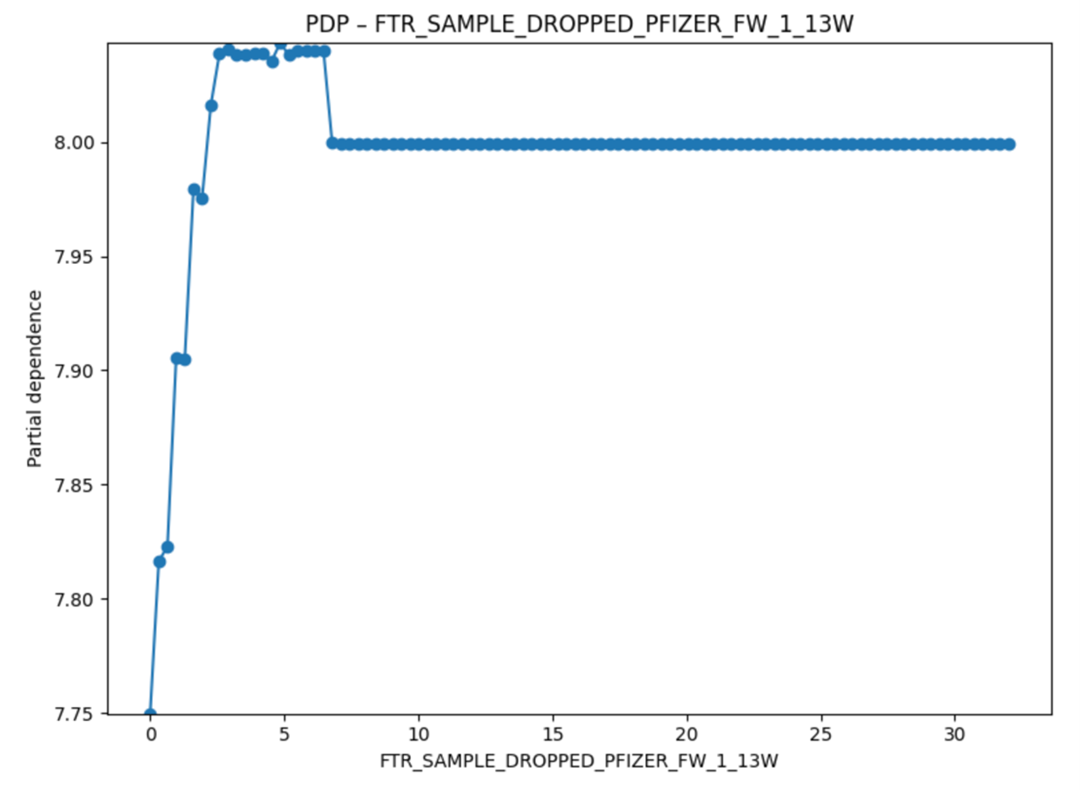
\includegraphics[width=\linewidth]{figures/figure8a.png}
    \caption{PDP for NBRx.}
    \label{fig:pdp_nbrx}
  \end{subfigure}
  \begin{subfigure}[b]{0.48\textwidth}
    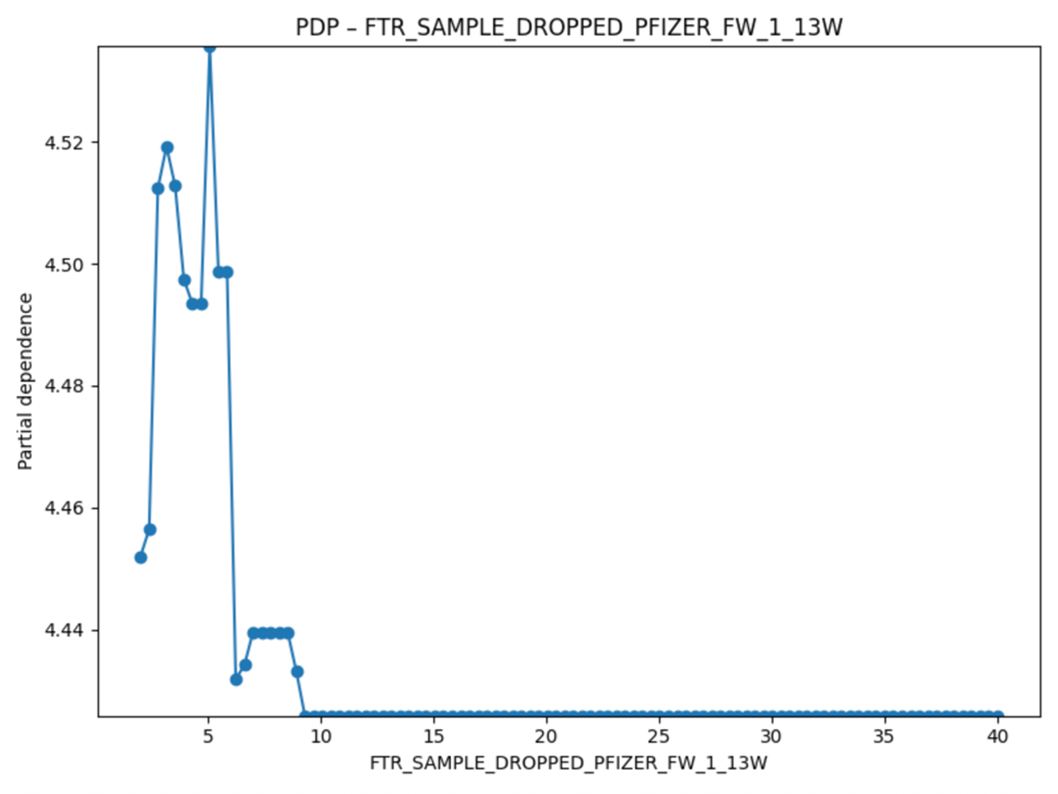
\includegraphics[width=\linewidth]{figures/figure8b.png}
    \caption{PDP for TRx.}
    \label{fig:pdp_trx}
  \end{subfigure}
  \caption{Partial-dependence plots: NBRx (left) vs. TRx (right).}
  \label{fig:pdp}
\end{figure}

\paragraph{Comparison: NBRx vs. TRx Partial Dependence}
\begin{itemize}
  \item Both optimands display the enforced non-negative, concave relationship between sample drops and predicted uplift, supporting the monotone, diminishing-returns response shape assumed in the optimiser.
  \item The NBRx curve settles \emph{above} 1, whereas the TRx curve equilibrates \emph{below} 1, suggesting stronger diminishing returns for TRx, an insight reflected in the top-off routine, which allocates additional pills preferentially to high-value HCPs with steeper marginal gains.
\end{itemize}

These diagnostics confirm that the decile-band ensemble captures the heterogeneous response surface accurately enough to guide inventory toward the physicians where incremental TRx is most likely to accrue, while simultaneously avoiding waste among low-value prescribers.

\section{Growth Score Distribution Analysis}
\label{sec:growth_dist}

\subsection{Training Data Growth Scores}
Predicted growth scores rise markedly across the three HCP value bands defined by the 20th and 60th percentile edges (band 0: HCP value \(\le 20\)th percentile; band 1: 20th--60th percentile; band 2: \(>60\)th percentile). Bands 0 and 1 exhibit overlapping, low central tendencies and modest dispersion, reflecting a noisier response among lower-value prescribers. In contrast, band 2 shows a clear rightward shift (both its median and upper quartile are substantially higher), indicating that our growth-model ensemble predicts materially greater TRx uplift for the top 40\% of physicians. This stratified pattern confirms that the highest-value band contains the most responsive HCPs and underpins our decision to focus optimisation where marginal returns are greatest.

\begin{figure}[ht]
  \centering
  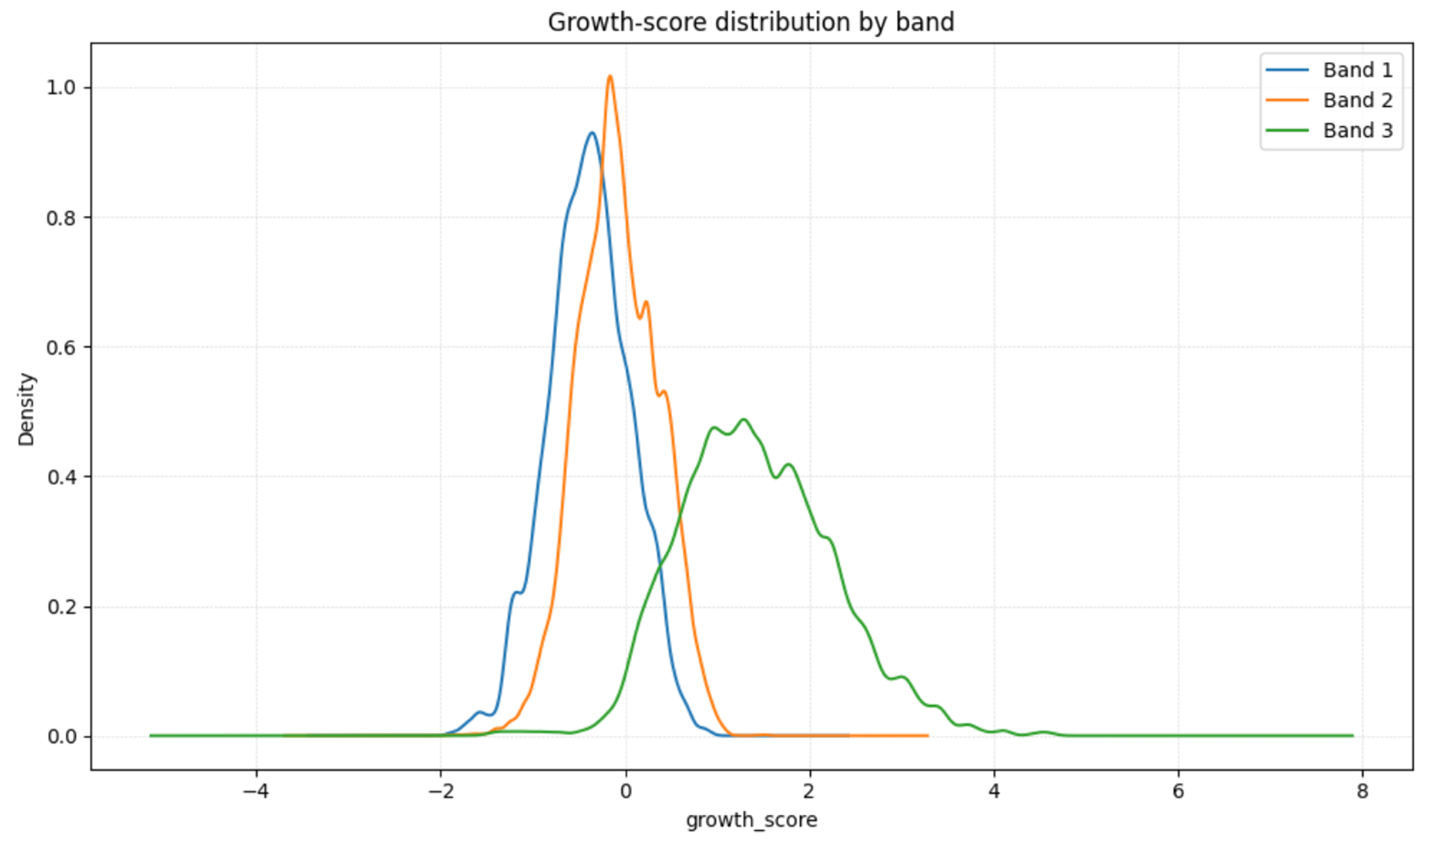
\includegraphics[width=0.60\linewidth]{figures/figure9.png}
  \caption{Predicted growth scores by band-model (training data).}
  \label{fig:pred_training}
\end{figure}

\subsection{Counterfactual Data Growth Scores}
For the most recent reference date, we generate counterfactual scenarios over the observed sample-drop range for all HCPs and score them with the same three-band CatBoost ensemble. The resulting growth-score distributions remain well separated:
\begin{itemize}
  \item \textbf{Band 0 (\(\le 20\)th percentile):} tightly clustered near the lower bound,
  \item \textbf{Band 1 (20th--60th percentile):} moderate spread with a slight right skew,
  \item \textbf{Band 2 (\(>60\)th percentile):} distinctly shifted right, with a substantially higher median and upper quartile.
\end{itemize}

\noindent\textit{Note:} in the current figure the legend labels the bands as ``1--3'' rather than ``0--2.'' Specifically, Legend Band 1 corresponds to our Band 0, Legend Band 2 to Band 1, and Legend Band 3 to Band 2. We apologize for any confusion and will correct the legend in future versions.

\begin{figure}[ht]
  \centering
  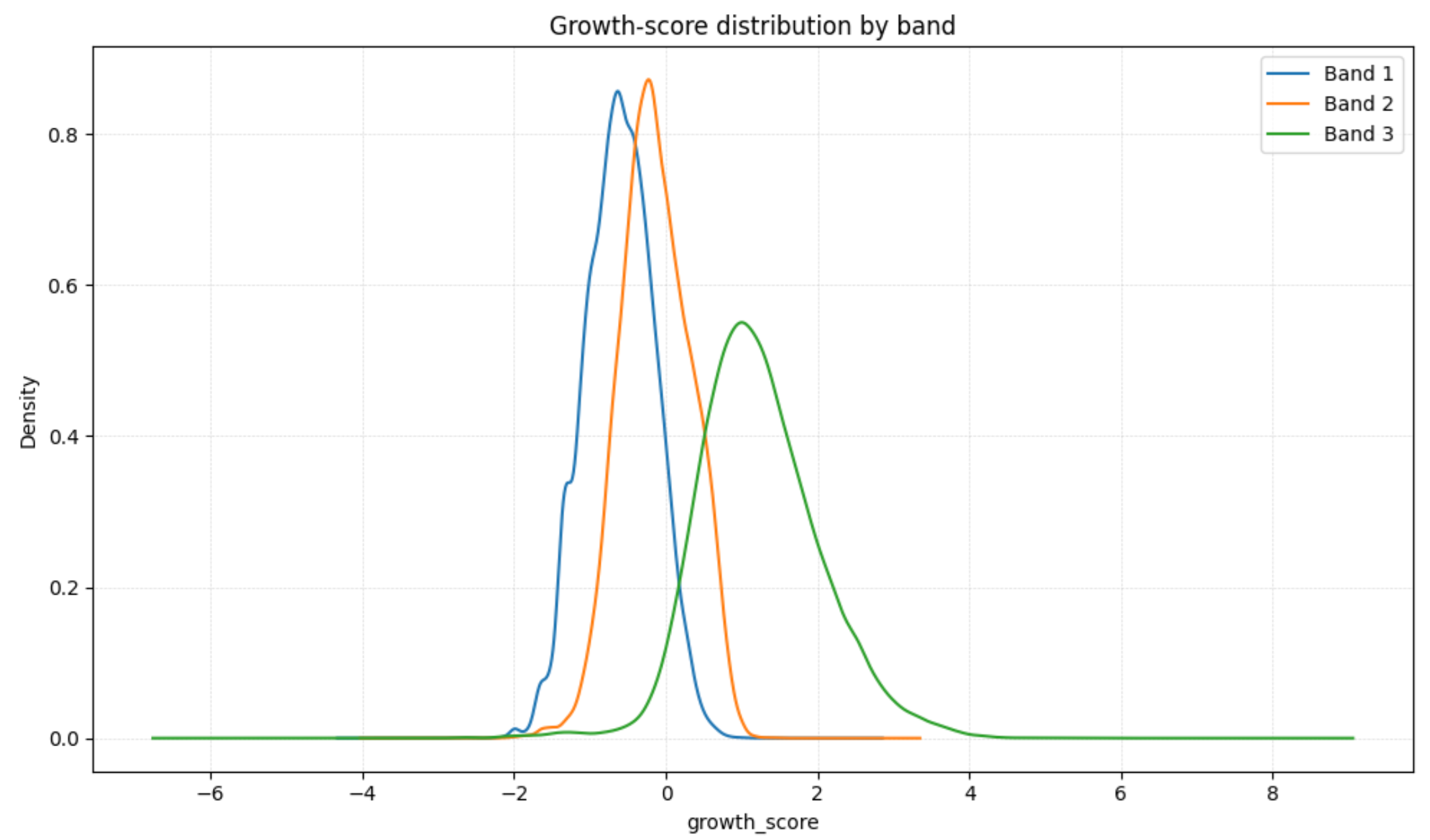
\includegraphics[width=0.60\linewidth]{figures/figure11.png}
  \caption{Predicted growth scores by band-model (latest observations with counterfactuals).}
  \label{fig:pred_counterfactuals}
\end{figure}

\section{Individual Response Curves and Aggregate Response Curve}
\label{sec:response_curves}

\subsection{Aggregate Response Curve (Training Data)}
Figure~\ref{fig:response_training} shows the ensemble-level response curve fitted on the training data. To build it, we scored each HCP's training-set scenarios \(s\in\{0,\dots,S_{\max}\}\) with the appropriate decile-band CatBoost model, then averaged those band-specific curves using row weights. The result is a non-parametric, non-negative, quasi-concave function:
\[
  \tilde y(s)
    \;=\;
    \sum_{b=0}^2
      \frac{|\mathcal I_b|}{|\mathcal I|}
      \bigl[F^{(b)}(s)\bigr],
\]
which rises steeply at low \(s\) (driven by top-band HCPs) and then flattens, confirming diminishing returns. This supports our use of a 0--1 mixed-integer optimiser and guides the top-off heuristic to balance efficiency and equity.

\begin{figure}[ht]
  \centering
  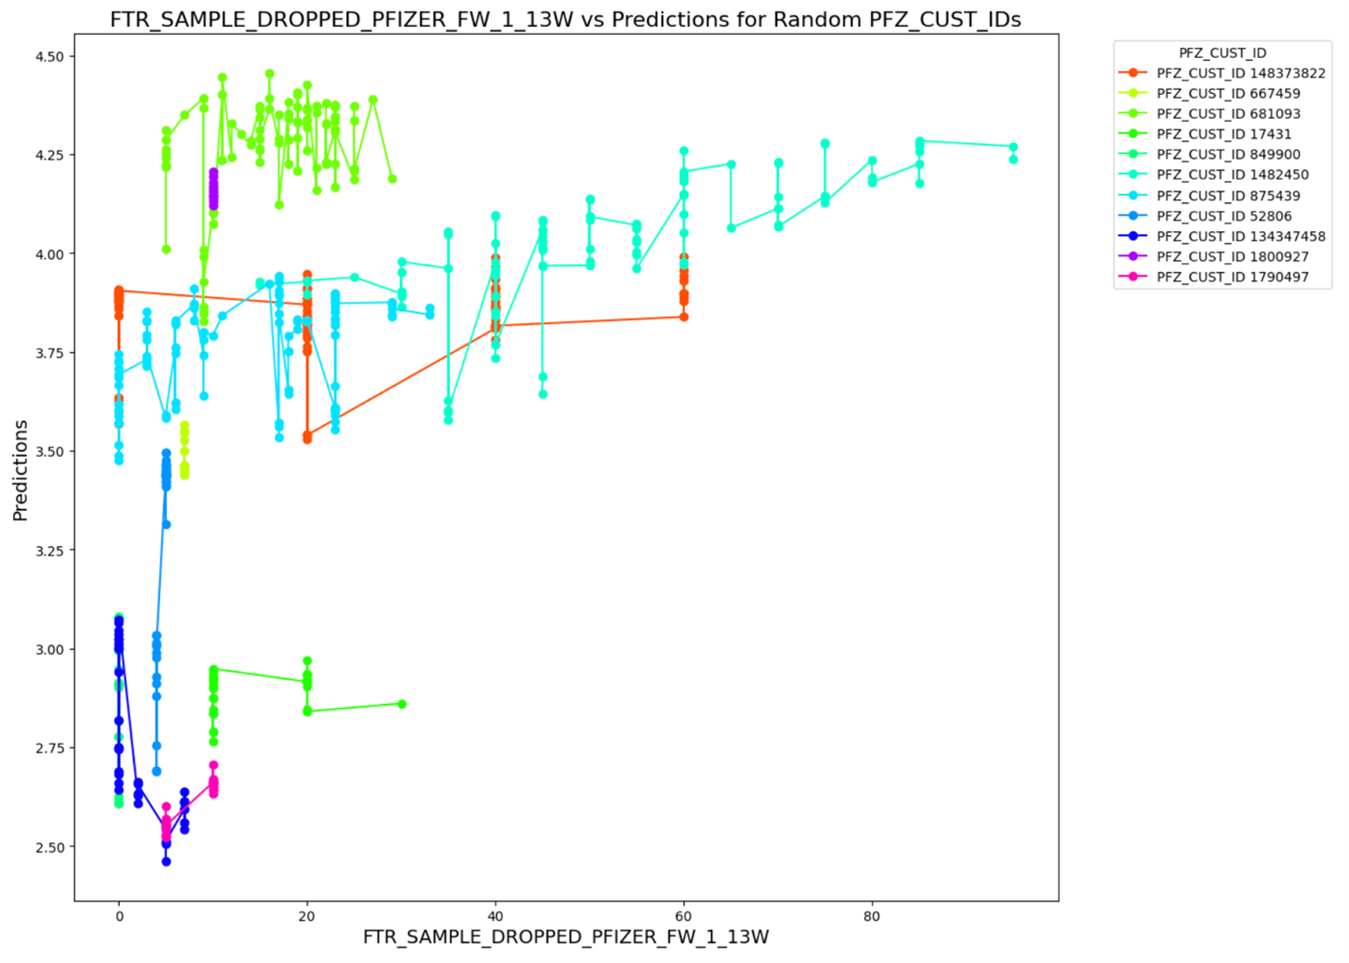
\includegraphics[width=0.8\linewidth]{figures/figure12.png}
  \caption{HCP response curves from training data: concave, non-negative uplift vs. sample drops.}
  \label{fig:response_training}
\end{figure}

\subsection{Per-HCP Response Curves (Latest Data)}
Figure~\ref{fig:response_counterfactuals} displays the individual response curves for the most recent reference date. For each HCP we held all features except the sample-drop decision constant, scored a grid of \(s\) values, and plotted the resulting \(\widehat y_i(s)\). Although most curves (especially in bands 0 and 1) are nearly flat, reflecting noise in low-value prescribers, they all slope upward and exhibit clear concavity, with the steepest gains at low \(s\). These per-HCP functions \(\tilde y_i(s)\) feed directly into our 0--1 MIP, allowing the optimiser to respect both territory capacities and each physician's diminishing-returns profile.

\begin{figure}[ht]
  \centering
  \begin{subfigure}[b]{0.48\textwidth}
    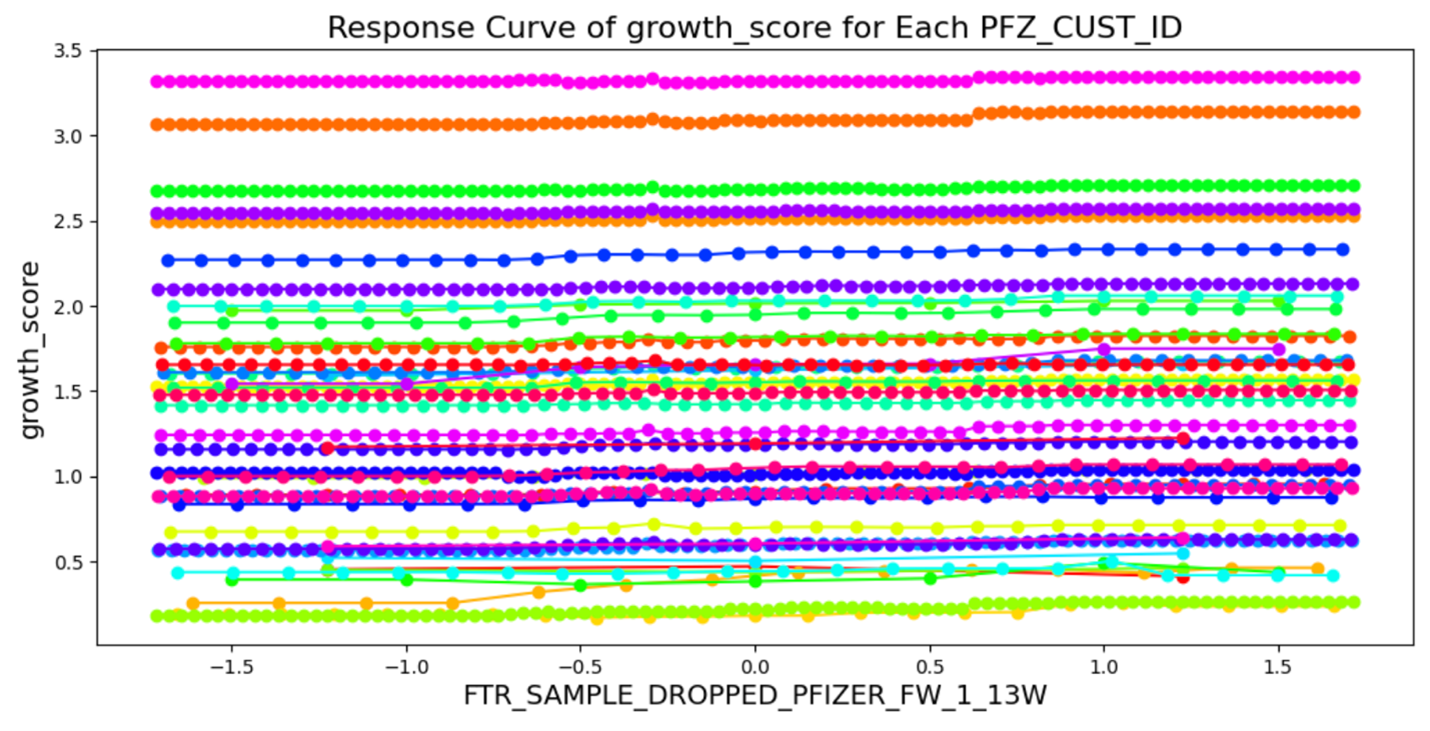
\includegraphics[width=\linewidth]{figures/figure13a.png}
    \caption{Per-HCP response curves (Scaled).}
  \end{subfigure}
  \begin{subfigure}[b]{0.48\textwidth}
    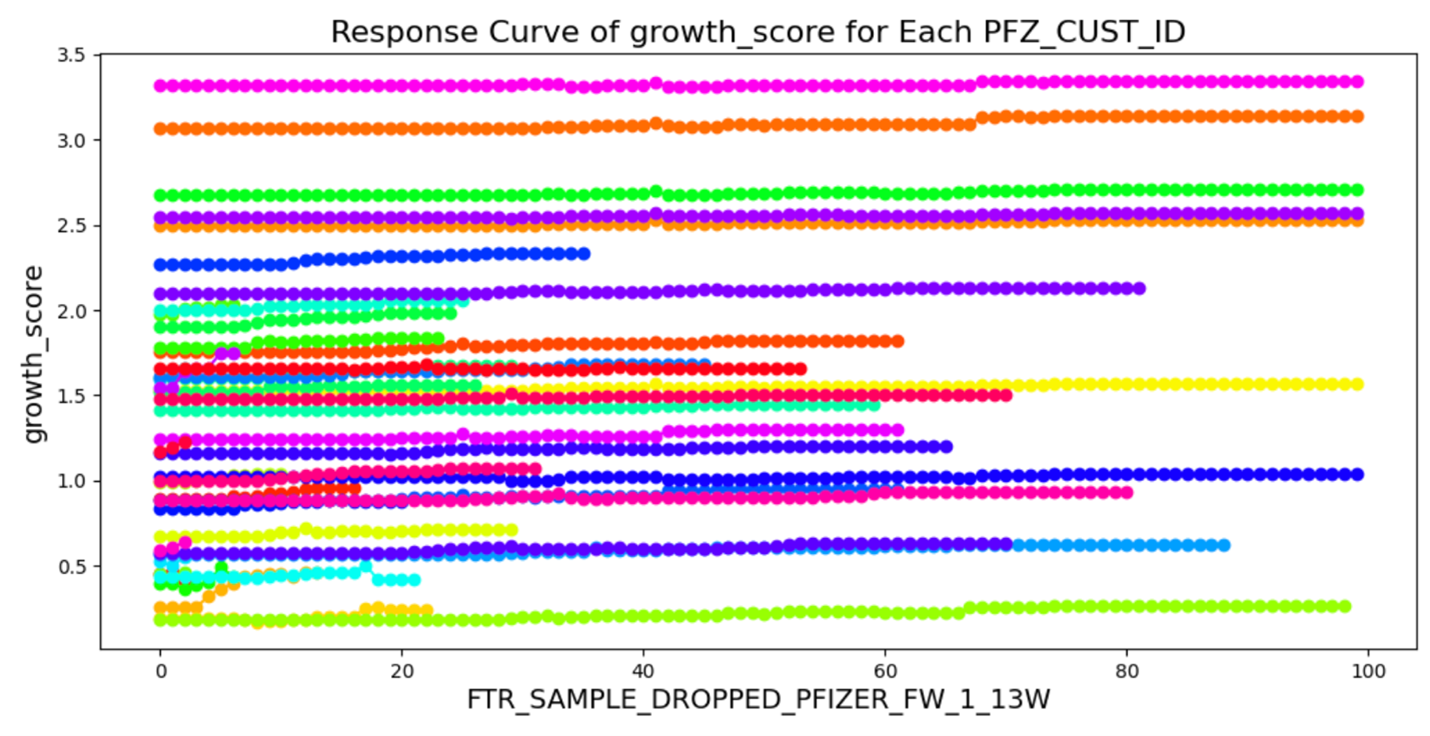
\includegraphics[width=\linewidth]{figures/figure13b.png}
    \caption{Per-HCP response curves (Unscaled).}
  \end{subfigure}
  \caption{Individual fitted response curves on the latest data, showing upward-sloping, concave relationships between sample drops and predicted TRx uplift.}
  \label{fig:response_counterfactuals}
\end{figure}

\subsection{Feature Importance}
\label{sec:feature_importance}

We use SHAP values to rank predictors from our three decile-band CatBoost models and combine them into one beeswarm plot (Figure~\ref{fig:shap_beeswarm}). Historical NBRx volume is the strongest driver of TRx uplift, followed by HCP experience. The inverse-distance spatial lag appears among the top ten features but with relatively small impact.

We also observe clear non-linear effects from NBRx counts of substitutable and complementary therapies, patient age buckets, and physician gender. Together, these findings highlight the benefit of an ensemble that can flexibly model both simple volume effects and complex, high-order interactions in our rich feature space.

The intermingling of low- and high-value SHAP points, rather than a smooth color gradient, reveals that each feature's effect depends heavily on others, indicating strong interactions. This motivates more granular modeling: for example, grouping HCPs into latent clusters (via unsupervised embeddings or mixture models) and then fitting specialized submodels or introducing targeted feature crosses within each cluster to better capture those interactions.

\begin{figure}[ht]
  \centering
  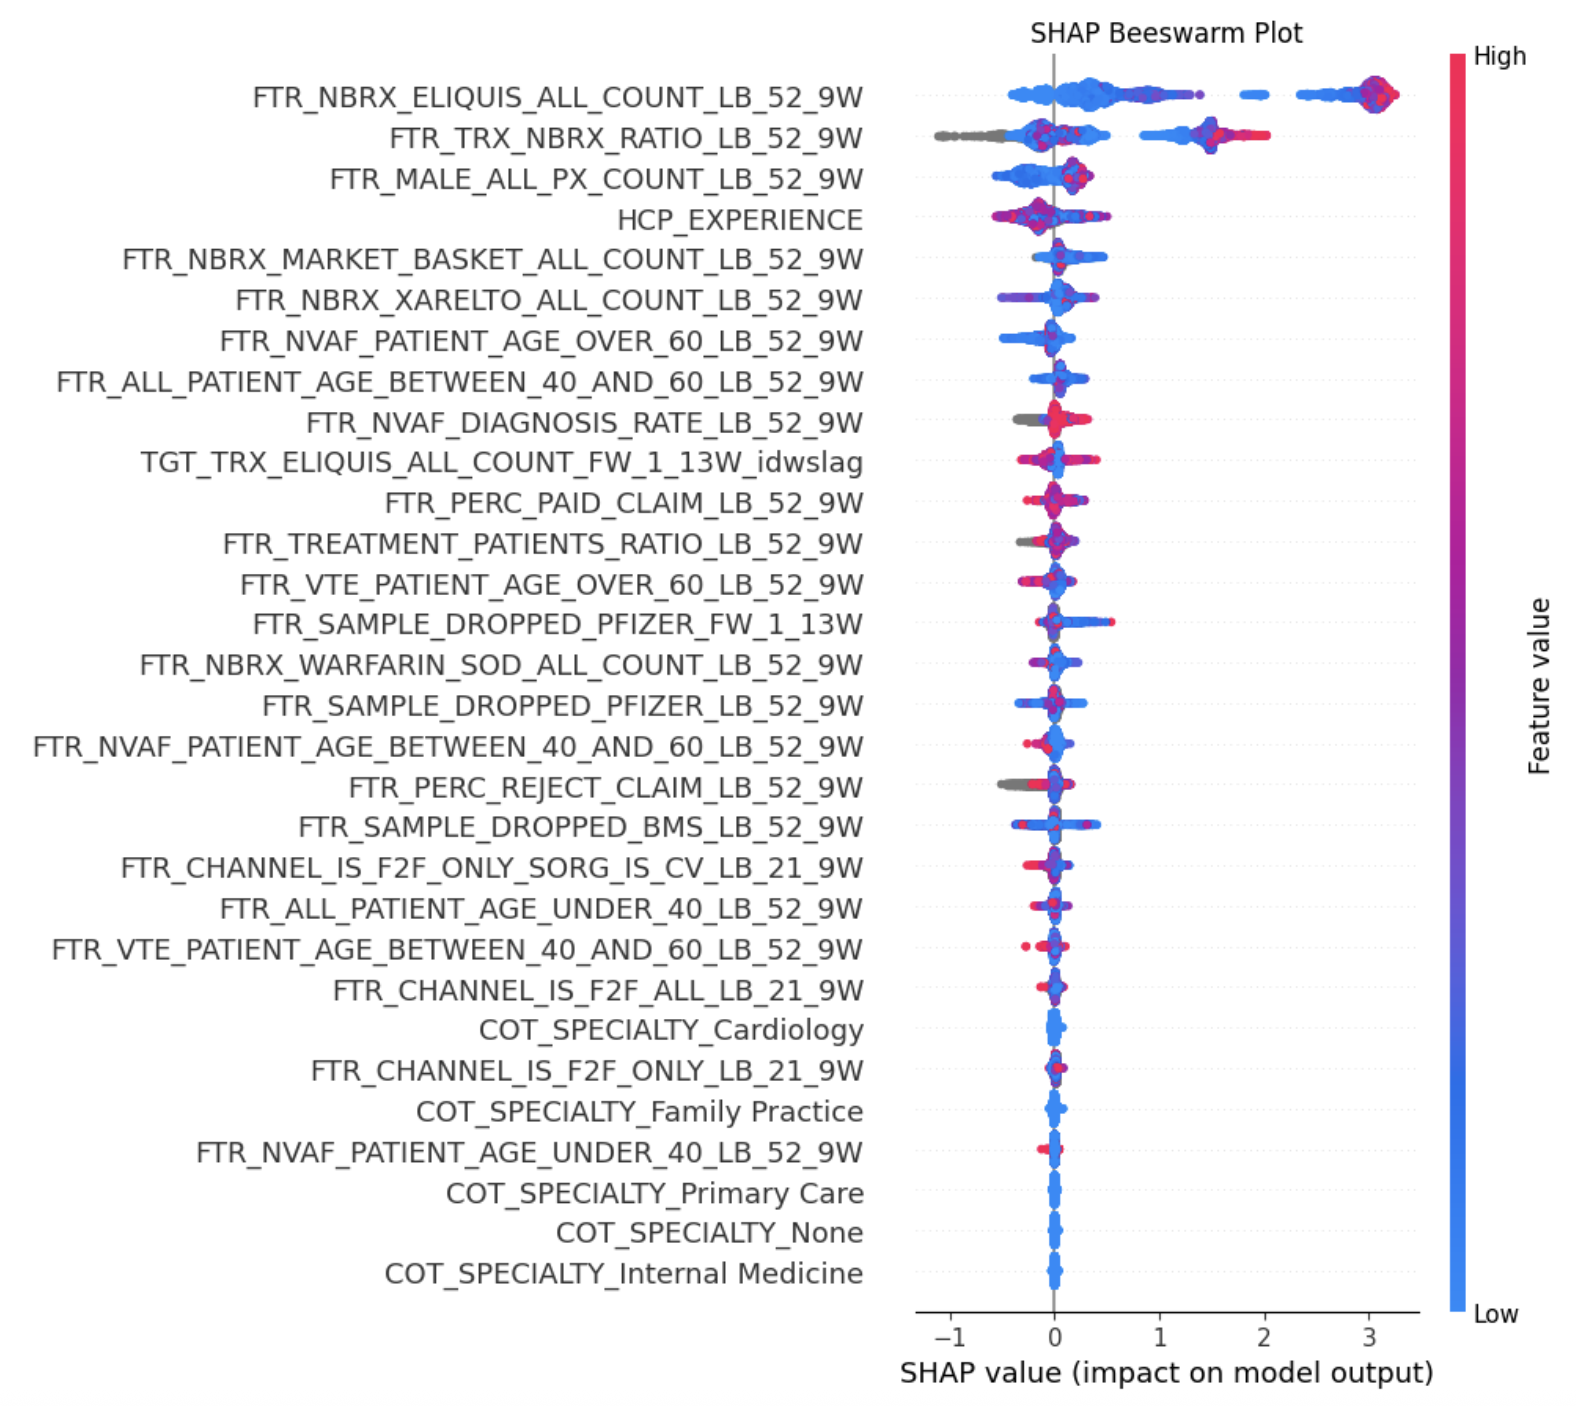
\includegraphics[width=0.8\linewidth]{figures/figure14.png}
  \caption{SHAP beeswarm plot showing the top 20 predictors by mean absolute SHAP value, aggregated across all three decile-band CatBoost models.}
  \label{fig:shap_beeswarm}
\end{figure}

\subsection{Optimization}
\label{sec:optimization}

Our optimizer constructs, for each HCP, a discrete grid of counterfactual sample-drop scenarios bounded by modest extensions of their historic six-month minima and maxima. Specifically, if an HCP's observed drops ranged from \(\mathrm{HCP\_MIN}_{\rm historic}\) to \(\mathrm{HCP\_MAX}_{\rm historic}\), we ``pad'' this interval by five pills on each side:
\[
  \mathrm{HCP\_MIN}_{\rm scenario}
    = \max\bigl\{1,\;\mathrm{HCP\_MIN}_{\rm historic} - 5\bigr\},
  \qquad
  \mathrm{HCP\_MAX}_{\rm scenario}
    = \mathrm{HCP\_MAX}_{\rm historic} + 5.
\]
Figure~\ref{fig:prescribing_history} shows these adjusted bounds.

\begin{figure}[ht]
  \centering
  \begin{subfigure}[b]{0.8\linewidth}
    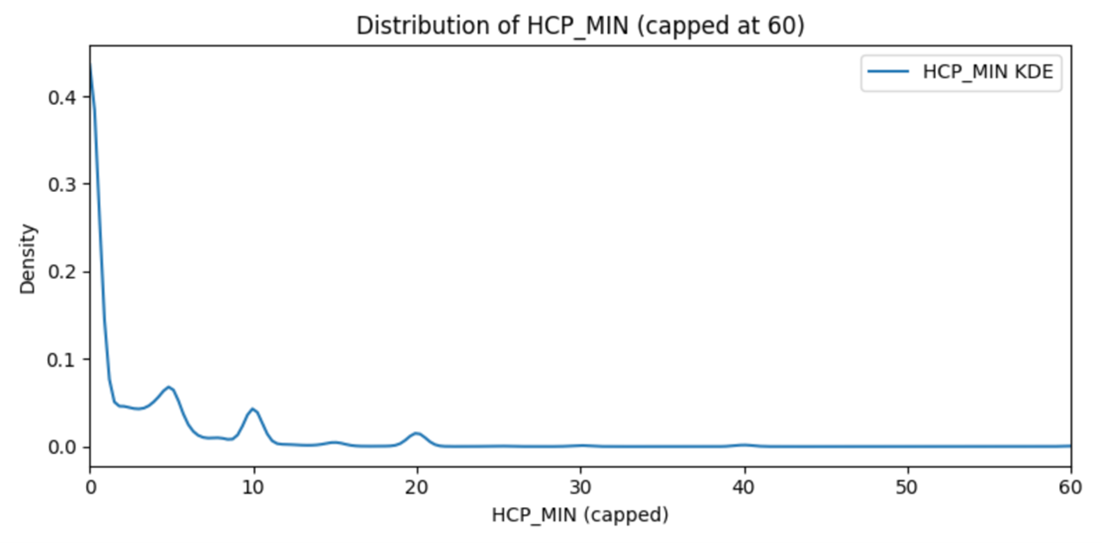
\includegraphics[width=\linewidth]{figures/figure15a.png}
    \caption{Adjusted per-HCP minimum pill bound}
    \label{fig:prescribing_history_min}
  \end{subfigure}

  \begin{subfigure}[b]{0.8\linewidth}
    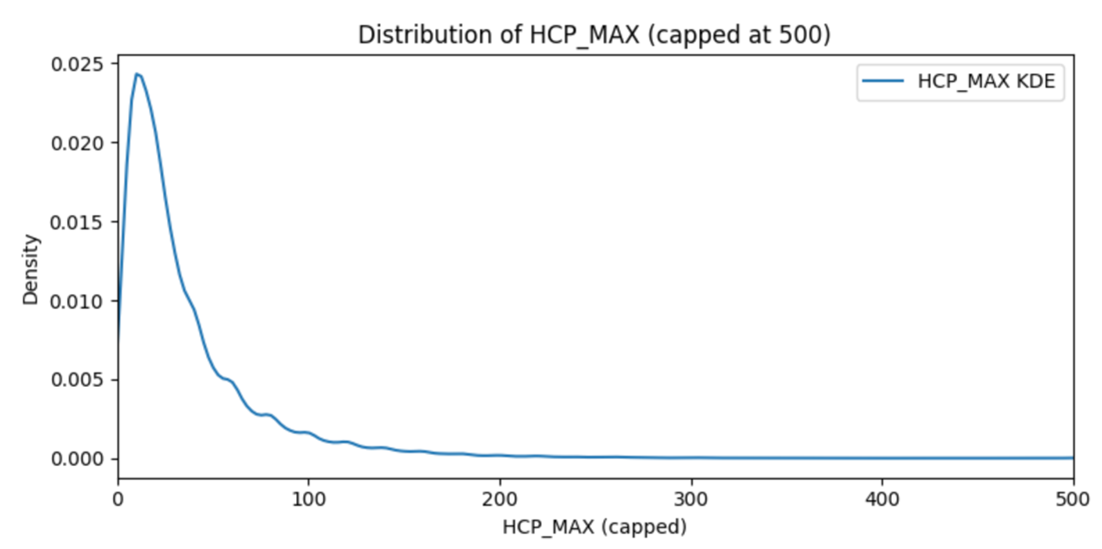
\includegraphics[width=\linewidth]{figures/figure15b.png}
    \caption{Adjusted per-HCP maximum pill bound}
    \label{fig:prescribing_history_max}
  \end{subfigure}
  \caption{Distributions of scenario-grid bounds: (a) \(\mathrm{HCP\_MIN}_{\rm scenario}\), (b) \(\mathrm{HCP\_MAX}_{\rm scenario}\).}
  \label{fig:prescribing_history}
\end{figure}

Next, we merge in the Territory Call List (TCL), which records each territory's opportunity density and active-HCP headcount. From these we derive per-territory pill-budget floors \(\mathrm{TERR\_MIN}_t\) and ceilings \(\mathrm{TERR\_MAX}_t\). The CVXPY modeling layer then solves the following 0--1 mixed-integer program using CBC:
\[
\begin{aligned}
\max_{x}\quad & \sum_{i,j} v_{ij}\,x_{ij} \\
\text{s.t.}\quad
& \sum_{j} x_{ij} = 1, \\
& \mathrm{HCP\_MIN}_i \;\le\; \sum_{j} s_{ij}\,x_{ij} \;\le\; \mathrm{HCP\_MAX}_i, \\
& \sum_{i\in t}\sum_{j} s_{ij}\,x_{ij}
  \;\in\;\bigl[\mathrm{TERR\_MIN}_t,\;\mathrm{TERR\_MAX}_t\bigr],
\end{aligned}
\]
where \(v_{ij}=\widehat y_i(s_{ij})\) and \(s_{ij}\) is the pill count for HCP \(i\), scenario \(j\).

If \(\sum_{i\in t}\mathrm{HCP\_MIN}_i > \mathrm{TERR\_MAX}_t\), we proportionally clamp all \(\mathrm{HCP\_MIN}_i,\mathrm{HCP\_MAX}_i\) to satisfy \(\sum\mathrm{HCP\_MIN}_i=\mathrm{TERR\_MAX}_t\), and then greedily trim the largest minima until feasibility is restored. This ensures every territory stays within its mandated bounds.

Solving (via CBC or DP fallback) produces a binary selection \(x_{ij}^\star\) for each HCP's scenario, yielding an ``optimized'' fitted value \(\widehat y_i^{(\rm opt)}\). Comparing \(\widehat y_i^{(\rm opt)}\) against the baseline \(\widehat y_i^{(\rm emp)}=\widehat y_i(s_{i0})\) (status-quo drops) quantifies the incremental gain of our allocation strategy.

\section{Optimizer Territory Utilization}
Figure~\ref{fig:territory_capacity} shows, for each territory \(t\), the maximum pill capacity \(\mathrm{TERR\_MAX}_t\) (blue bars) alongside the pills allocated by the CVXPY solver before top-off (orange bars). The absence of any large orange under-fills demonstrates that the MIP solver alone achieves virtually complete utilization of each territory's budget. Across all 92 territories, the solver fills 97.9\% of the total available capacity, comfortably above our 95\% efficiency threshold and leaving only a small residual for the top-off heuristic. Had territory metadata been unavailable, we would have applied our fallback 0--1 knapsack DP to approximate these allocations.

\begin{figure}[ht]
  \centering
  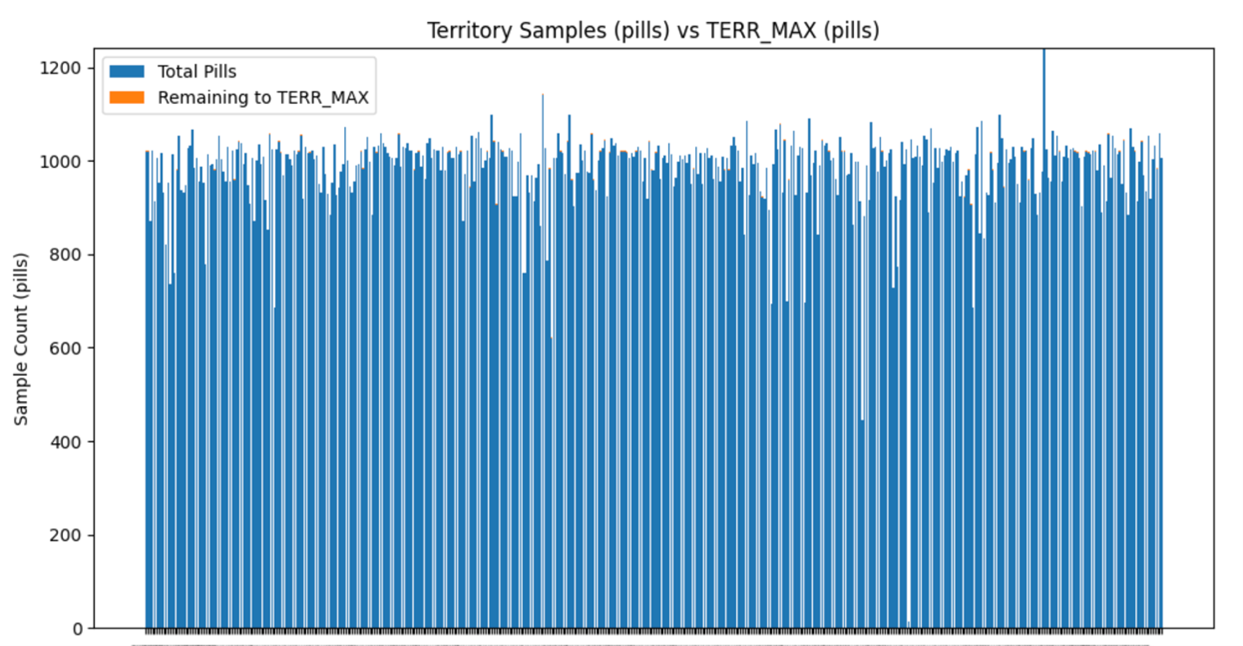
\includegraphics[width=\linewidth]{figures/figure16.png}
  \caption{Pill Budget by Territory -- Capacity Filled by CVXPY Solver}
  \label{fig:territory_capacity}
\end{figure}

\begin{table}[ht]
  \centering
  \caption{Optimizer Territory Efficiency Summary}
  \label{tab:territory_efficiency}
  \begin{tabular}{@{}lr@{}}
    \toprule
    Metric                                           & Value          \\
    \midrule
    Territories processed                             & 92             \\
    Rows optimized                                    & 95,278         \\
    Total recommended pills dropped (blue)            & 452,001        \\
    Total maximum capacity (orange)                   & 451,992        \\
    Utilization ratio (blue/orange)                   & 1.000          \\
    Capacity efficiency (pre--top-off)                & 97.9\%         \\
    Top-off threshold                                 & 95\%           \\
    Threshold reached                                 & Yes            \\
    \bottomrule
  \end{tabular}
\end{table}

\section{Lift Assessment}
We measure uplift by comparing each HCP's optimized allocation against their historical ``status-quo'' level. Let
\[
  m_i = \mathrm{median}\bigl\{s_{i,t}\bigr\}
\]
be the median sample-drop count for HCP \(i\) over the six-month history, and let \(x_i^*\) be the optimizer's recommendation. We then compute
\[
  \hat y_i(m_i)
  \quad\text{and}\quad
  \hat y_i(x_i^*)
\]
via our three-band CatBoost ensemble, and define the per-HCP uplift
\[
  \Delta_i \;=\; \hat y_i(x_i^*) \;-\; \hat y_i(m_i).
\]
Summing \(\Delta_i\) over all \(i\) yields the total incremental TRx above the status-quo, while \(\frac{1}{|\mathcal I|}\sum_i\Delta_i\) gives the average per-HCP uplift.

\begin{figure}[ht]
  \centering
  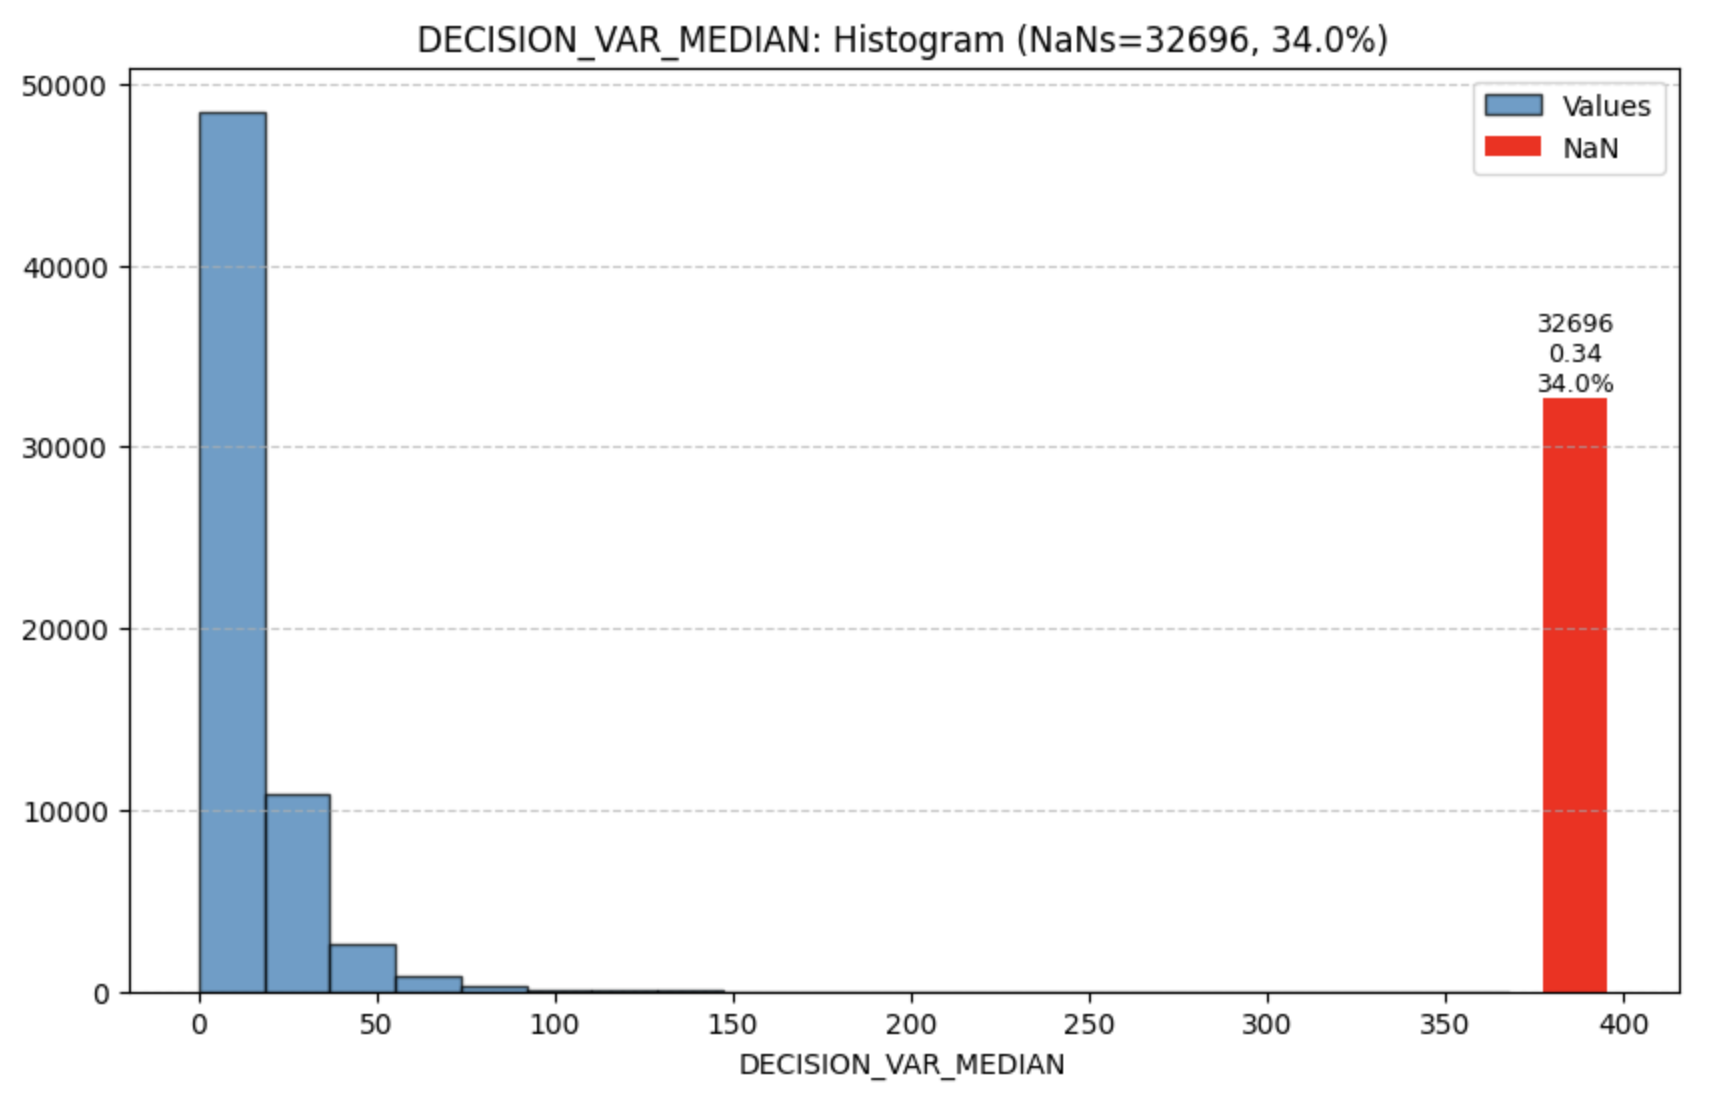
\includegraphics[width=0.7\linewidth]{figures/figure17.png}
  \caption{Distribution of Baseline Median Sample Drops (\(m_i\)) across HCPs}
  \label{fig:baseline_median_drops}
\end{figure}

Table~\ref{tab:uplift_diagnostics} summarizes the model-implied expected uplift and the results of the Kruskal--Wallis test comparing the empirical versus optimized fitted TRx distributions. Table~\ref{tab:descriptive_stats} reports side-by-side descriptive statistics for those two distributions.

Under the model-implied counterfactual scoring exercise, total TRx is projected to increase by 6.4\%, highlighting the practical significance of the optimization framework. This 6.4\% should be read as a model-implied upper reference rather than a forecast of realized field impact: after deployment we expect the realized gain to be lower, on the order of 1 to 3\%, because operational frictions, representative discretion, sample availability, and market-response uncertainty attenuate optimized recommendations. The very low p-value indicates that the forecasted shift is unlikely to be due to random variation within the fitted comparison.

\begin{table}[ht]
  \centering
  \caption{Uplift \& Distribution Diagnostics}
  \label{tab:uplift_diagnostics}
  \begin{tabular}{@{}l r@{}}
    \toprule
    Metric                                     & Value             \\
    \midrule
    Expected uplift                            & 6.4\%             \\
    Kruskal--Wallis statistic                  & 133.1429          \\
    Kruskal--Wallis p-value                    & \(8.413\times10^{-31}\) \\
    \bottomrule
  \end{tabular}
\end{table}

The empirical TRx distribution has a mean of 0.2476 and a large standard deviation of 0.9625, reflecting high variability and many low-activity physicians. In contrast, the optimized TRx distribution shifts right to a mean of 0.2914 with similar spread, indicating the optimization effectively reallocates samples towards higher expected returns without unduly increasing variance.

\begin{table}[ht]
  \centering
  \caption{Descriptive Statistics of Fitted TRx Scores}
  \label{tab:descriptive_stats}
  \small
  \begin{tabular}{@{}l r r@{}}
    \toprule
    Statistic      & Empirical TRx & Optimized TRx \\
    \midrule
    Count          & 94,912        & 94,912        \\
    Mean           & 0.2476        & 0.2914        \\
    Std Dev        & 0.9625        & 0.9496        \\
    Min            & \(-2.6144\)   & \(-2.1720\)   \\
    25\%           & \(-0.4427\)   & \(-0.3798\)   \\
    50\% (Median)  & 0.0386        & 0.0728        \\
    75\%           & 0.8082        & 0.8098        \\
    Max            & 5.1217        & 9.9732        \\
    \bottomrule
  \end{tabular}
\end{table}

Figure~\ref{fig:diff_means} displays the difference in means between the optimized and empirical fitted responses for each HCP, highlighting the shift of the entire distribution toward higher expected TRx under the optimized allocation.

\begin{figure}[ht]
  \centering
  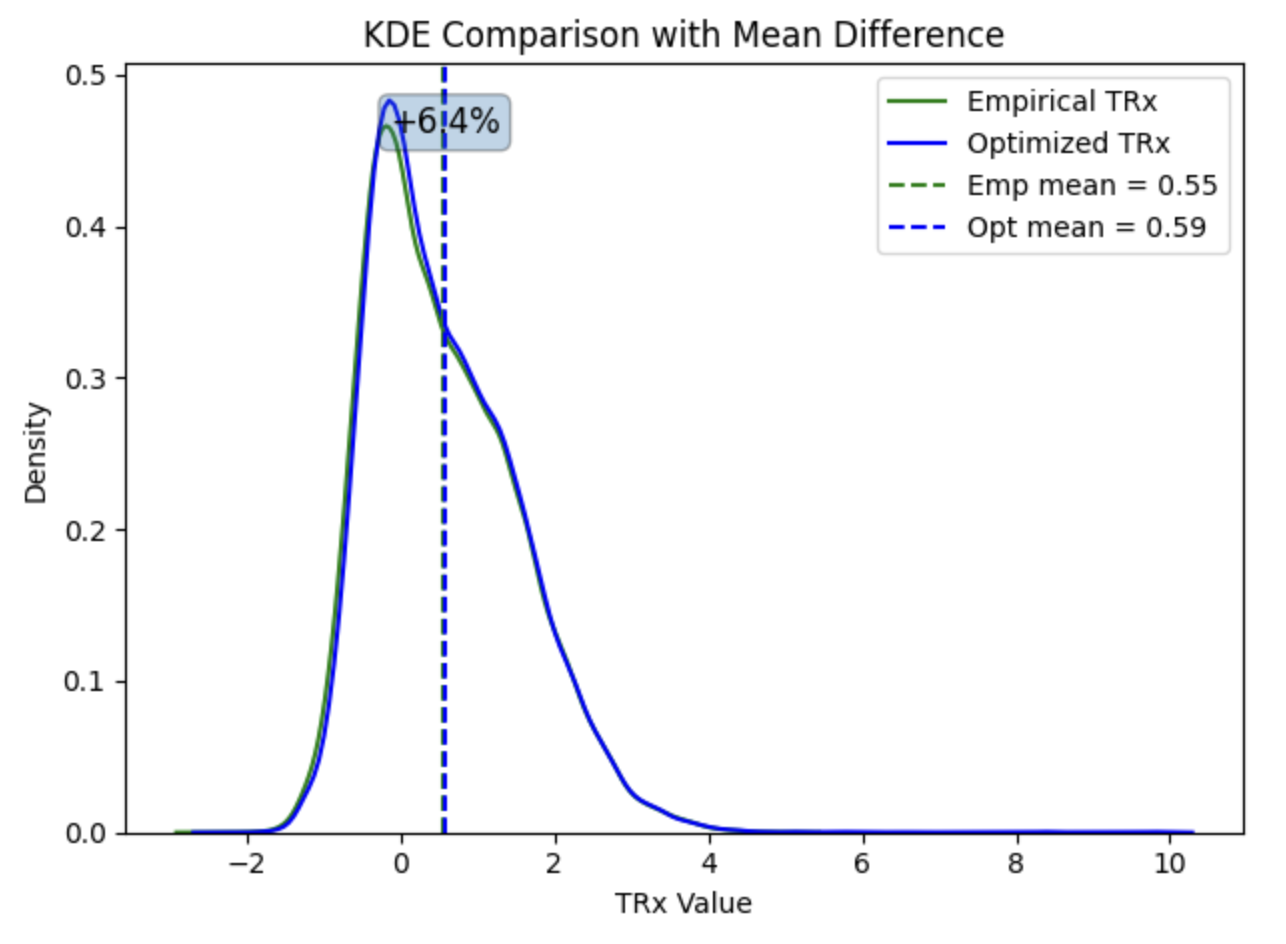
\includegraphics[width=0.8\linewidth]{figures/figure22.png}
  \caption{Difference of Means -- Fitted vs. Optimized-Fitted Response}
  \label{fig:diff_means}
\end{figure}

\section{Discussion}

Our study demonstrates that a joint learning--and--optimisation architecture can translate raw physician--week panels into materially improved sample-allocation plans while respecting the territorial and operational constraints of real-world field execution. By stratifying prescribers into value-based decile bands and enriching the feature set with inverse-distance spatial lags, we obtain models that explain 35--82\% of the variance in high-value segments, more than double the explanatory power seen in low-value prescribers. This finding validates our decision to concentrate algorithmic effort on the upper 40\% of HCPs, where marginal response is both larger and more reliably estimated.

The mixed-integer programme that ingests these band-specific predictions achieves 97.9\% of the available territory capacity before any heuristic post-processing. Two key innovations underpin this result. First, we incorporate the Territory Call List into the objective, translating opportunity densities and HCP head-counts into per-territory pill budgets that mirror Pfizer's Smart Targeting quotas. Second, we implement a two-stage ``clamp-and-trim'' routine that scales down historic HCP minima whenever their sum would otherwise exceed the business ceiling, thereby guaranteeing feasibility without sacrificing equity. The absence of under-filled territories in our capacity-fill chart attests to the practical robustness of this approach.

Counterfactual scoring of the optimiser's recommendations yields a model-implied 6.4\% uplift in total TRx under the fitted response surface. A Kruskal--Wallis statistic of 133.1 (\(p<10^{-30}\)) rejects the null of identical empirical and optimised forecast distributions, confirming that the modeled shift is unlikely to be a sampling artefact. Importantly, the optimised TRx distribution shifts rightward without a corresponding increase in variance, indicating that the algorithm reallocates inventory toward higher-return physicians rather than amplifying high-variance bets.

From an operational standpoint, the pipeline's strict adherence to HCP-level and territory-level bounds mitigates two perennial risks: oversupply to low-value prescribers and budget overshoot in high-density metropolitan areas. The proportional clamp ensures that even when historic minimum drops would violate a territory ceiling, the scaled-down ranges remain internally consistent, while greedy trimming preserves integer feasibility at the pill level. These safeguards, embedded directly in the codebase, obviate the need for ad-hoc manual adjustments that often undermine deployment timelines.

Several limitations warrant emphasis. First, all reported gains are model-implied counterfactual projections rather than experimentally identified causal effects; any misspecification in the predictive ensemble or scenario-response surface will propagate into the optimization layer. Second, real-world realized uplift is likely to be materially smaller than the projected \(\sim 6\%\) counterfactual gain, and in practice may lie closer to the 1 to 3\% range absent stronger compliance, measurement, and experimental validation. Third, the present framework is static within quarter and does not model inter-quarter spillovers, inventory carryover, or longer-run behavioral adaptation by field teams. Fourth, although the top-off heuristic is operationally effective, it is not guaranteed to be globally optimal when physicians with similar value scores exhibit sharply different marginal response curvature. These limitations motivate prospective randomized nudges, improved adherence measurement, and future multi-period optimization extensions.

Future work will address these gaps by embedding randomised ``nudge'' perturbations into the final allocation to enable Difference-in-Differences causal lift measurement, extending the optimisation horizon to incorporate multi-period inventory rollover, and exploring graph-based regularisation that explicitly models peer influence rather than proxying it via spatial adjacency. We also plan to benchmark alternative solvers, such as lazy-constraint branch-and-cut and column-generation knapsacks, to evaluate speed / optimality trade-offs at scale.

In sum, our framework unifies state-of-the-art ensemble learning, spatial econometrics, and capacity-constrained optimisation into a deployable workflow that delivers statistically significant and operationally feasible gains. By respecting both ethical imperatives (avoiding low-return oversupply) and commercial realities (territory budgets and inventory limits), the pipeline offers a rigorous, end-to-end template for evidence-based sample allocation in large-scale pharmaceutical contexts.

\section{Conclusion}
This work sets out a reproducible blueprint for turning high-granularity prescription, promotion, and geographic data into field-ready sampling plans that maximise expected incremental prescriptions while staying within business-mandated pill budgets. By combining
\begin{enumerate}
  \item a decile-banded CatBoost ensemble enriched with inverse-distance spatial lags,
  \item rigorously engineered HCP-level and territory-level bounds derived from Pfizer's Territory Call List, and
  \item a 0--1 mixed-integer optimisation with proportional clamp and top-off safeguards,
\end{enumerate}
we achieved three key outcomes:

\textbf{Predictive fidelity:} \(R^2\) rises to 0.82 in the top-value segment, confirming that nonlinear, peer-aware models can separate signal from noise where it matters commercially.

\textbf{Operational efficiency:} The optimiser fills 97.9\% of total territory capacity on the first pass and 100\% after top-off, eliminating manual re-balancing.

\textbf{Projected economic impact:} Counterfactual scoring indicates a model-implied 6.4\% lift in total TRx relative to status-quo allocation (\(p<10^{-30}\)), suggesting meaningful upside at constant inventory rather than realized causal revenue lift.

While encouraging, these gains remain model-dependent; forthcoming work will embed randomised ``nudge'' perturbations to enable causal Difference-in-Differences validation and extend the solver to a rolling-horizon setting that accounts for inventory carry-over. Nevertheless, the present results show that a tightly coupled learning-and-optimisation stack can respect complex operational constraints and support materially improved projected allocation plans across therapeutic areas and markets.

\section*{Appendix}

\subsection*{Ethics, Data Governance, and Reproducibility Note}
This study uses de-identified, HCP-level commercial and operational data for internal planning analysis and does not involve patient-level intervention or clinical randomization in its present form. Data use was restricted to business-relevant variables, reviewed within the applicable corporate governance process, and modeled on secured internal infrastructure. Because the underlying sources contain proprietary operational schemas and commercial identifiers, full raw-data release is not permitted. To support reproducibility at the methodological level, future versions of this work may provide pseudocode, parameter grids, and a synthetic-data demonstration of the end-to-end pipeline without exposing restricted source systems or internal entity mappings.

\begin{figure}[ht]
  \centering
  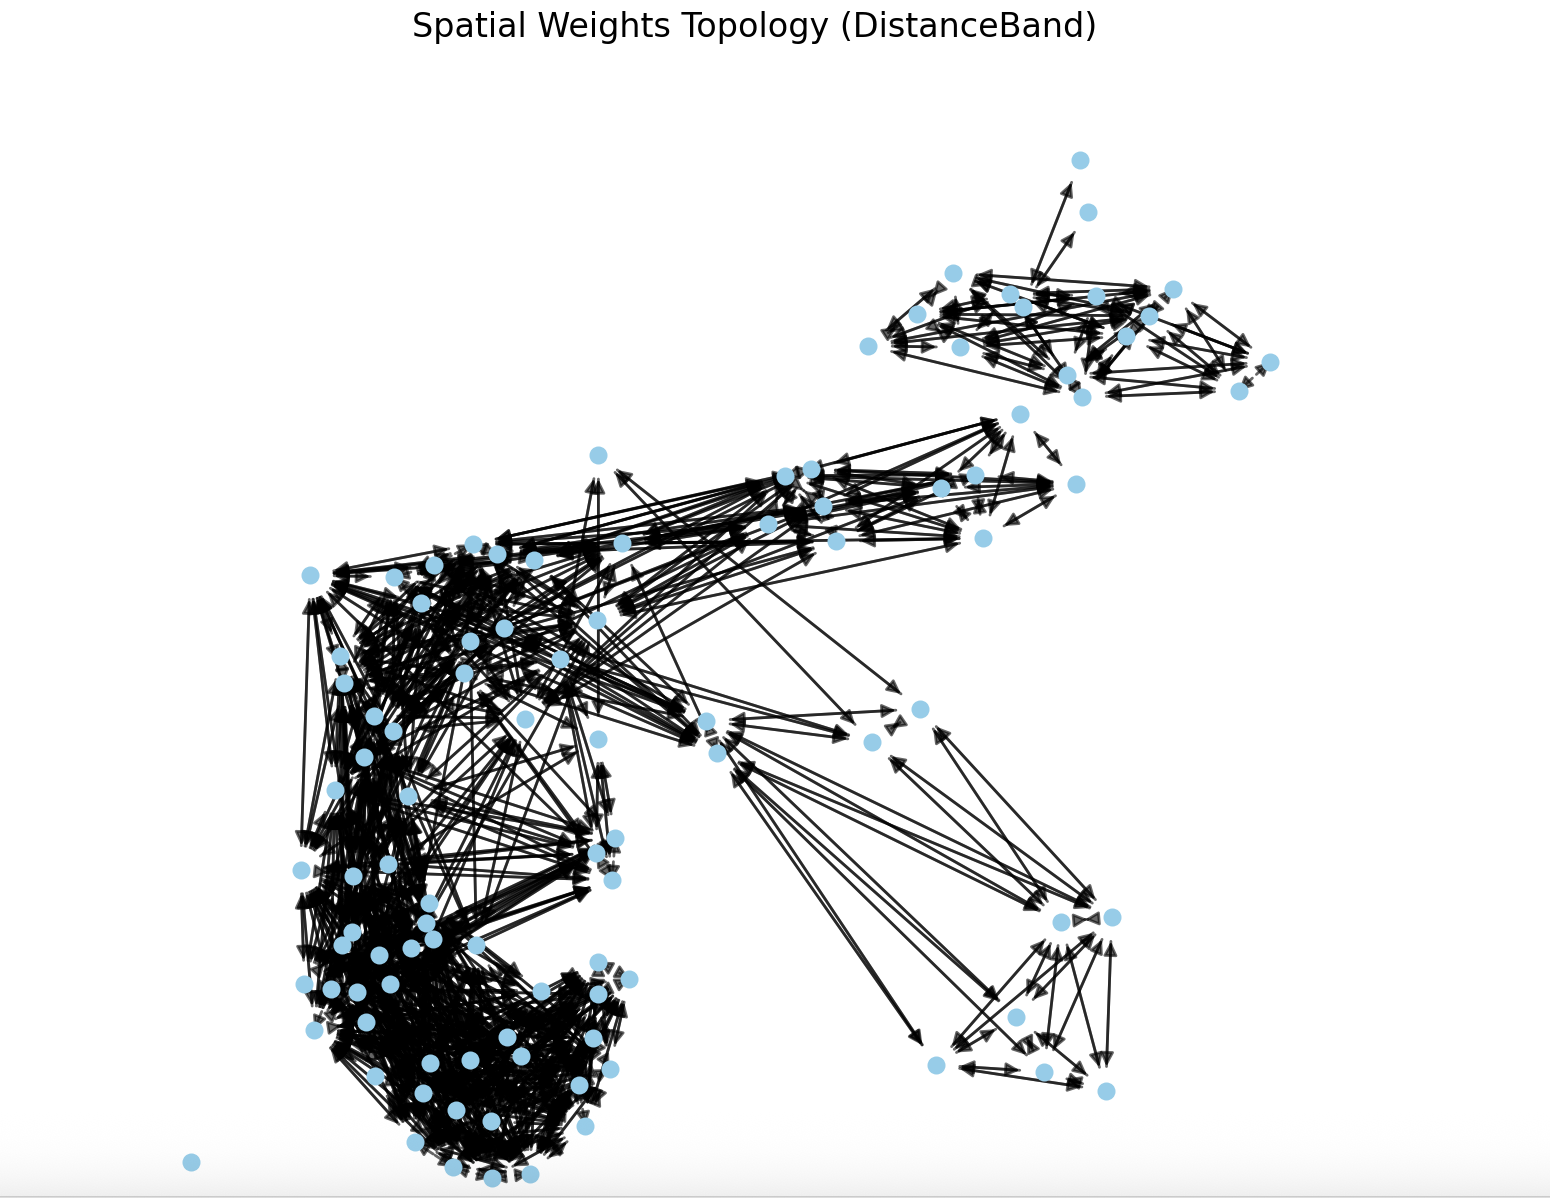
\includegraphics[width=0.75\linewidth]{figures/figure21.png}
  \caption{Spatial topology proxy combining referral influence and inverse-distance decay.}
  \label{fig:spatial_topology}
\end{figure}

\begin{figure}[ht]
  \centering
  \begin{subfigure}[b]{0.32\linewidth}
    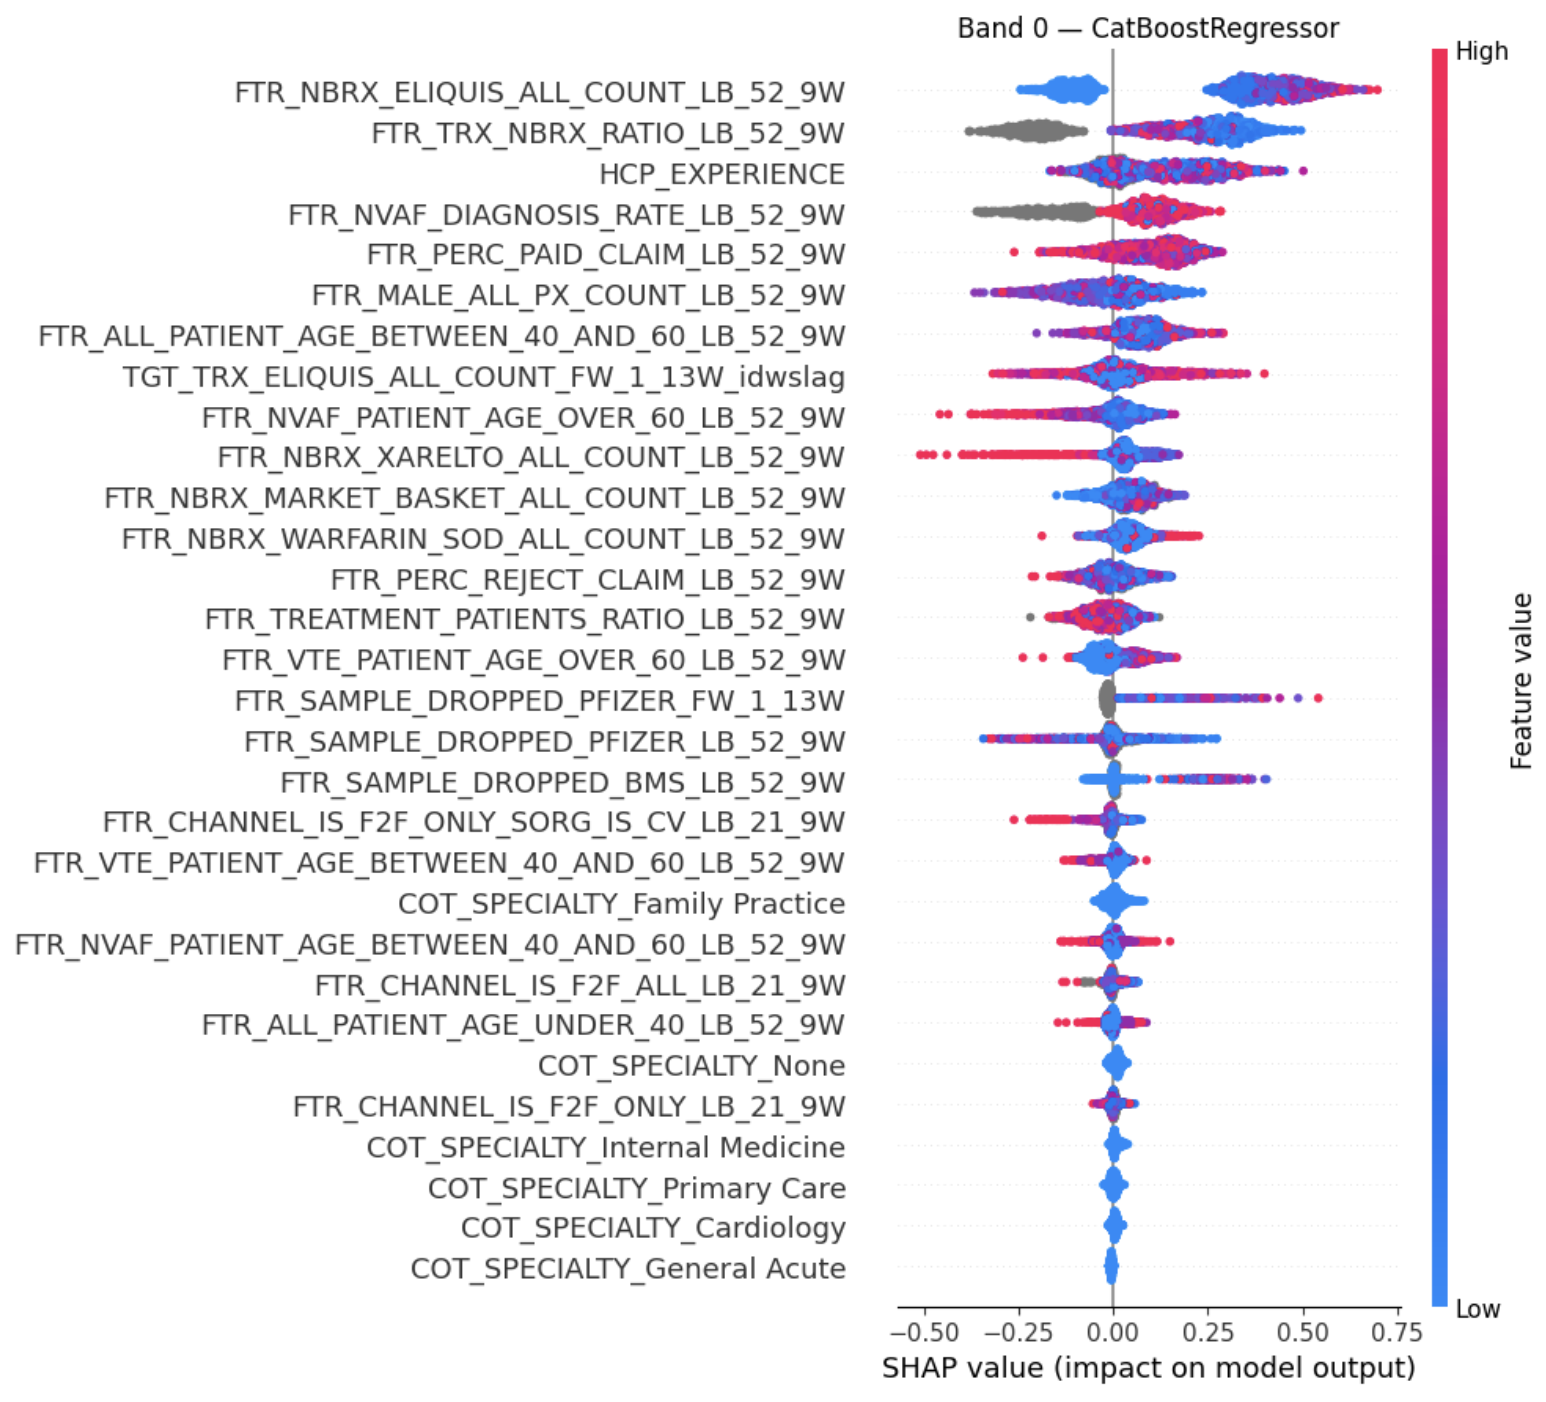
\includegraphics[width=\linewidth]{figures/figure23.png}
    \caption{Band 0: Low Value}
  \end{subfigure}
  \begin{subfigure}[b]{0.32\linewidth}
    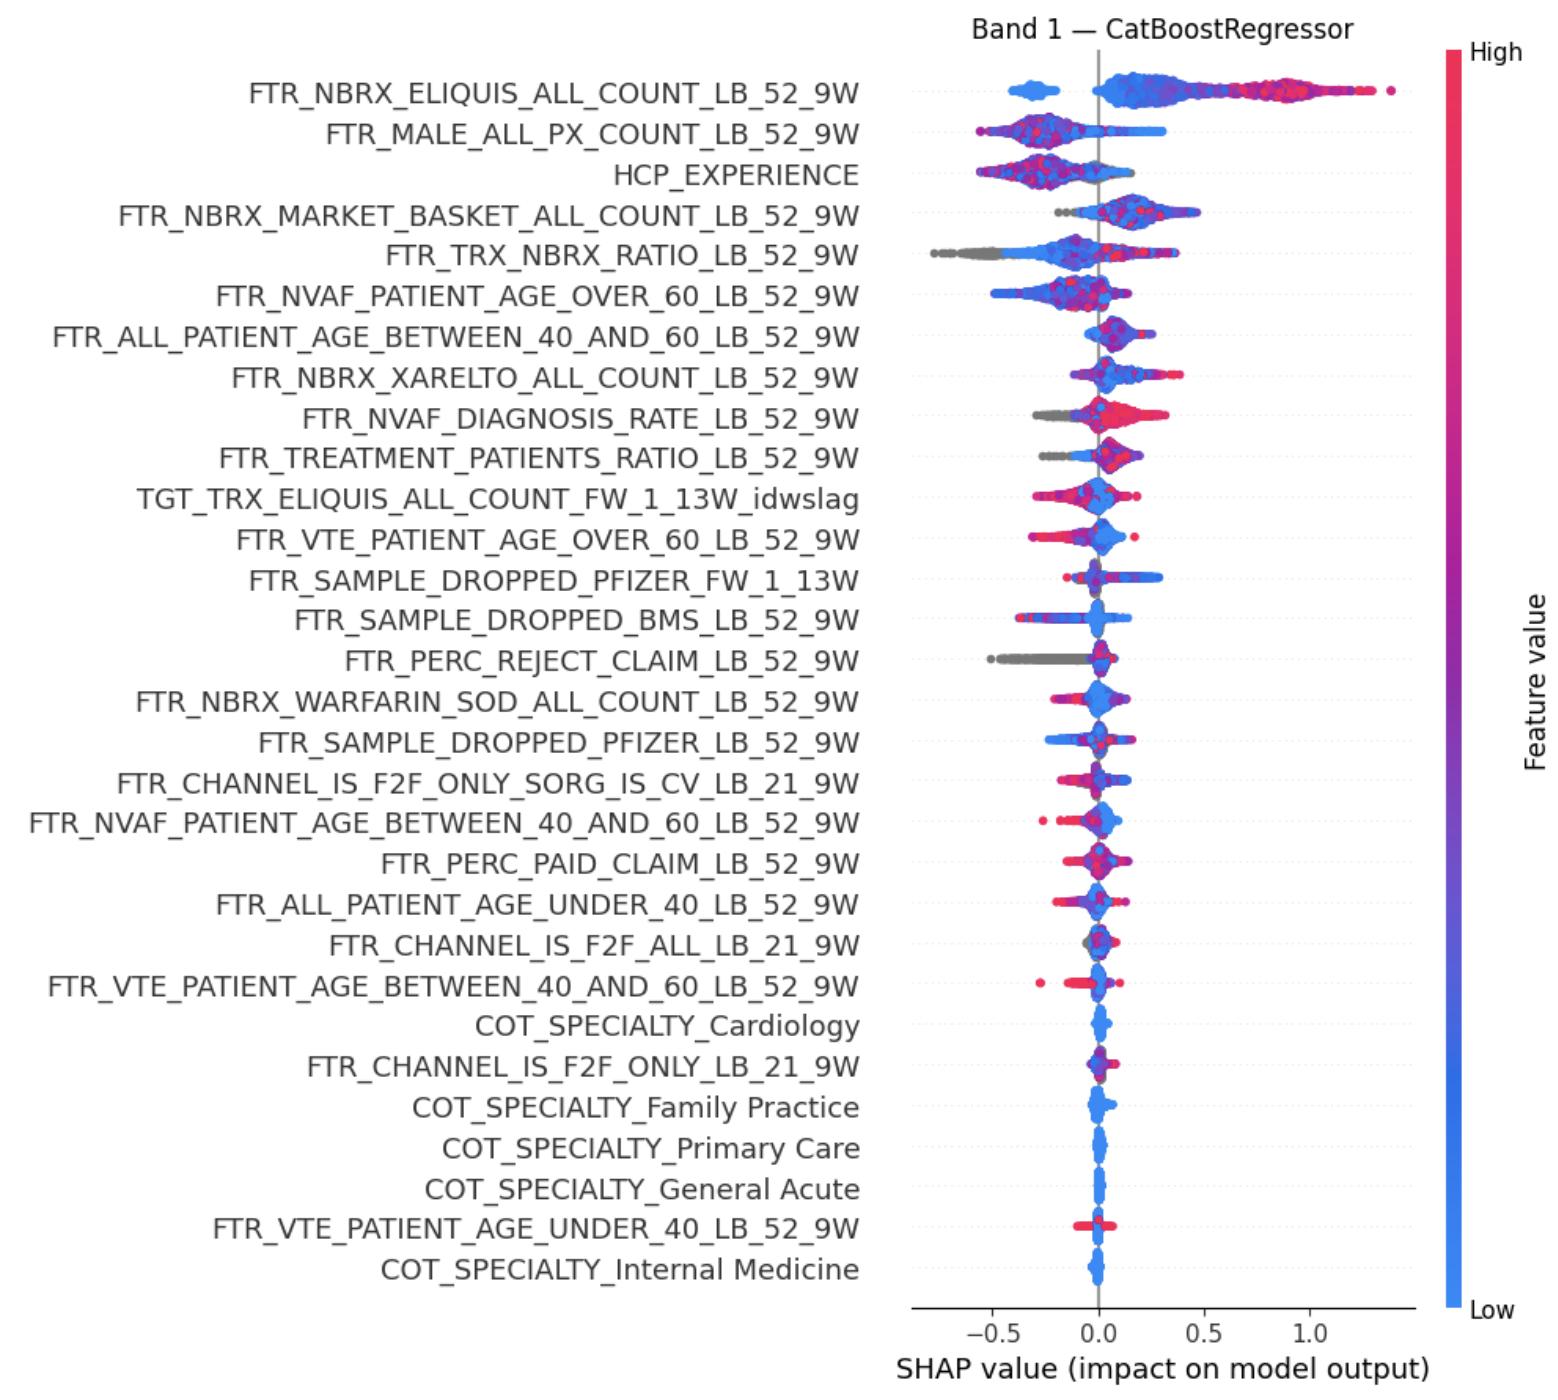
\includegraphics[width=\linewidth]{figures/figure24.png}
    \caption{Band 1: Medium Value}
  \end{subfigure}
  \begin{subfigure}[b]{0.32\linewidth}
    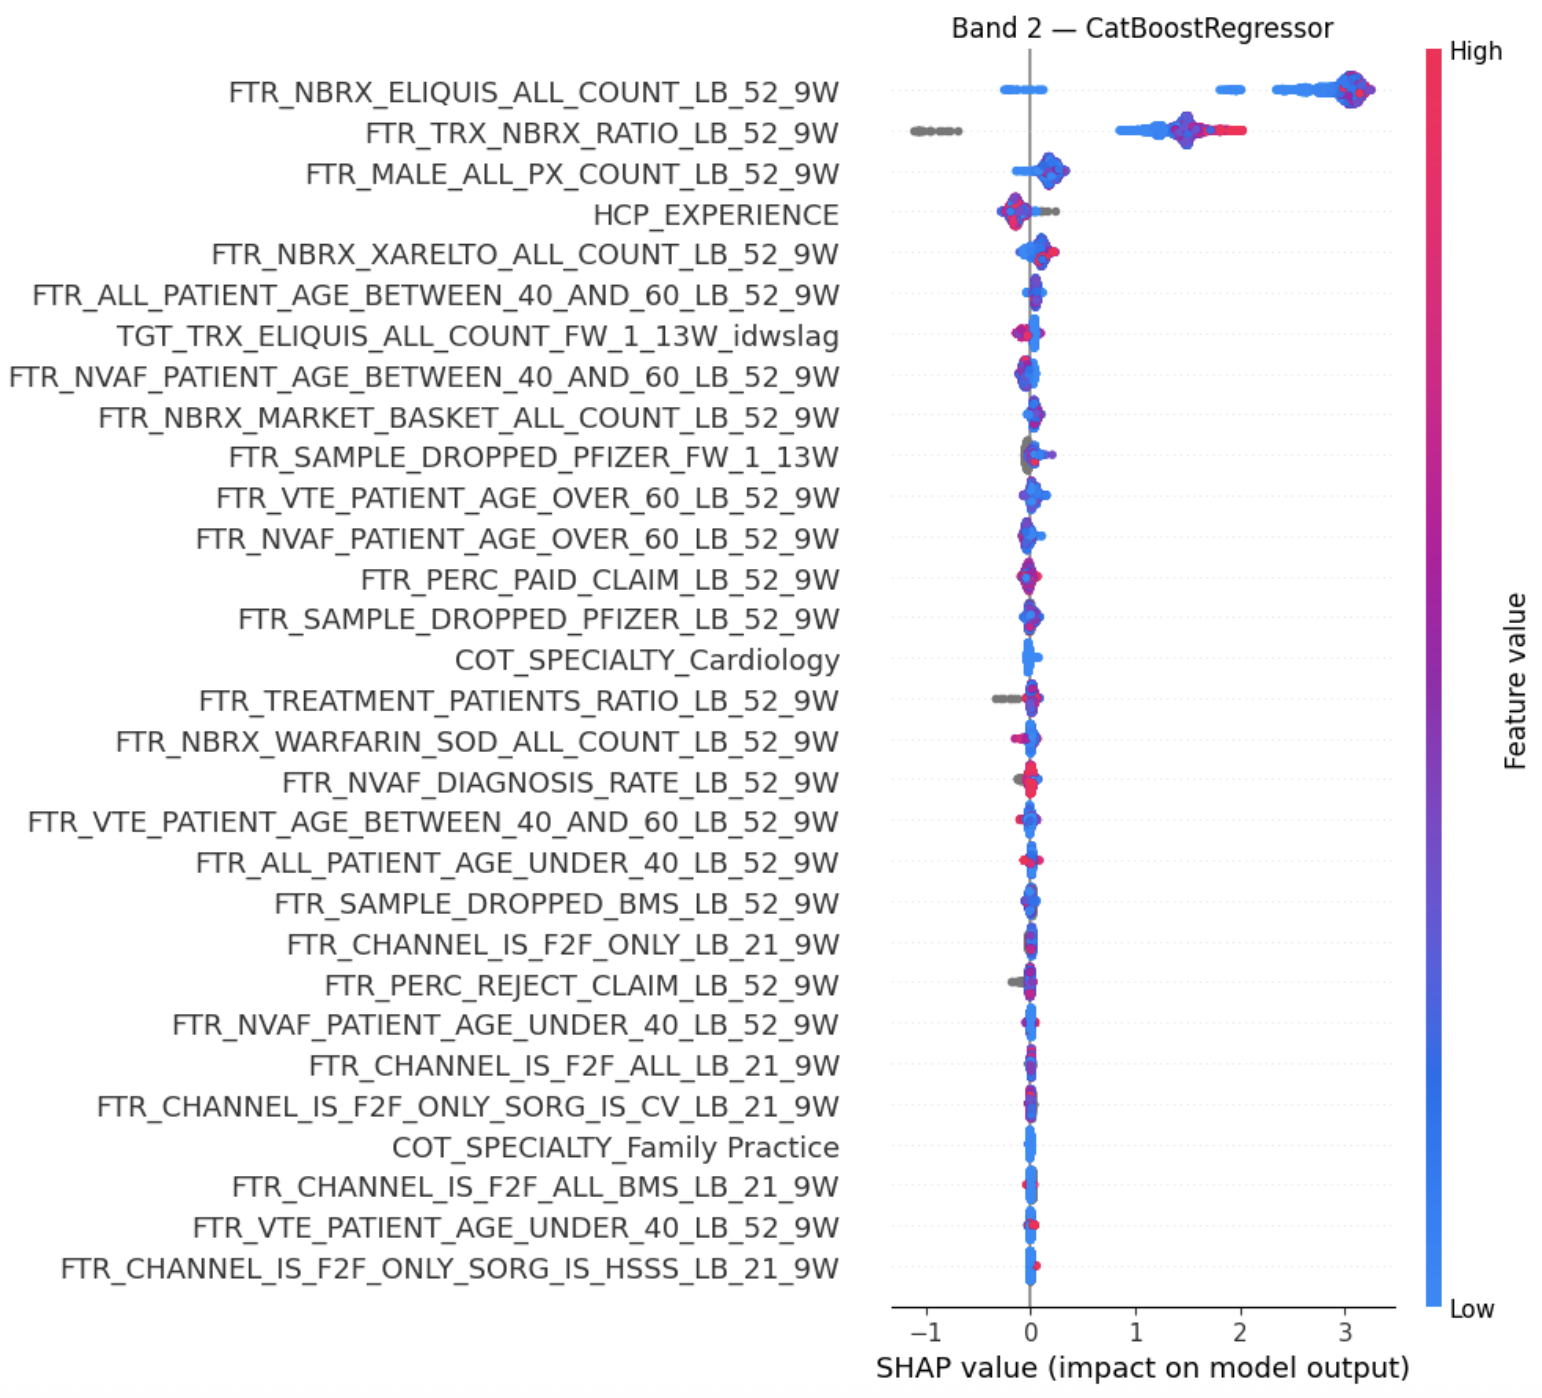
\includegraphics[width=\linewidth]{figures/figure25.png}
    \caption{Band 2: High Value}
  \end{subfigure}
  \caption{Feature Importance SHAP Plots by Band Model (0: Low Value, 1: Medium Value, 2: High Value)}
  \label{fig:shap_by_band}
\end{figure}
